\chapter{Fences - The economics of connectivity in spatial renewable resources}
%\footnote{I am grateful to Lauriane Mouysset and Christopher Costello, Martin Quaas, Giorgio Fabbri, Francesco Ricci, Valentin Cocco, Jérôme Pivard, Lucas Vivier, Romain Fillon, Alexandre Adrian (from Platt Vineyard),  as well as seminar participants at BINGO, the 2024 FAERE PhD Workshop, 2024 Parisian PhD Seminar in Environmental Economics for their helpful comments.}}
\interfootnotelinepenalty=100

%To fragment or thin : 


\begin{minipage}{0.9\textwidth}
\singlespace
%This article discusses the complex interplay between ecological conservation and economic activities within spatially distributed networks. Renewable ressources, such as game, and invasive species on land can be managed through their stock, and landscape connectivity. This article examines how overharvesting (or under in the case of an invasive species) and habitat fragmentation can be jointly managed. Spatial connectivity can be managed to solve the tragedy of the commons and lead to efficient harvest as property rights are secured. Nonetheless, fragmenting habitat can be detrimental, and a trade-off emerges between efficient harvesting and optimal fencing. This article examines the optimal management of spatially distributed, endogenously connected renewables. In a setting where economic and biological conditions are heterogeneous and positively correlated, efficient management leverages a spatial arbitrage opportunity, promotes habitat connectivity, and optimizes welfare. With negative correlations, efficient management implies not changing what Nature has done, and harvest rules need to be enforced for welfare maximization. On the other hand, I look at the dynamic game that emerges when players can choose their harvest level and how their land connects to others. I show, under mild conditions, that the non-cooperative equilibrium results in fragmented habitat but halts overexploitation. In some cases, it can result in optimal management, depending on the underlying heterogeneous economic and biological conditions. Moreover, observed ecosystem dynamics can be partly rationalized through economic factors. For instance, observed sink-source dynamics may reflect heterogeneous biological productivities, and environmental features, but also heterogeneous returns to species in non-cooperative equilibria. 
%Finally, I  examine which policies should be implemented in a second-best framing, where connectivity or harvesting policies can be implemented, and rank policy options across heterogenous landscapes. 
%This article contributes to the literature on optimal renewable management and brings the fishery literature back on land, as connectivity can be managed. It contributes to the dynamic network formation games literature in the context of a renewable resource. I emphasize the need for policies that consider the interconnectedness of ecological systems and the different margins of economic activities that impact them, aiming for sustainable management practices that ensure both ecological integrity and economic viability.
%It explores how optimal resource management changes with endogenous connectivity. Moreover, as connectivity can be changed, the extent of spatial externalities can be limited. This article highlights conditions where solving the spatial externality is the first best scenario instead of leveraging what Nature has rightfully done. 

This article examines the management of spatially distributed renewable resources—specifically wildlife and infectious diseases—through the lens of economic and spatial analysis. I focus on "bads" like invasive species and diseases, which cause economic and ecological harm, and utilize population control and fencing as central  mechanisms. I analyze how fencing influences resource flow and connectivity. On the one hand, in the presence of ecological and economic heterogeneities, fencing can be used to leverage spatial artbitrage opportunities. On the other hand, while promoted as a tool to incentivize the internalization of costs associated with ``bads", they may undo what Nature has rightfully done. In this sense, while fencing may be welfare improving in a setting with initially poor connectivity, an uncoordinated use of fencing, although welfare improving, is not welfare maximizing. The study develops a theoretical model that integrates aspects of stock and patch connectivity management and explores both cooperative and non-cooperative management strategies. The findings indicate that optimal management often requires a nuanced understanding of the spatial dynamics and economic costs associated with different control strategies. We present a series of propositions that characterize the conditions under which fencing and resource control strategies can be optimized, including the interaction effects of exclusionary and trap effects. This article contributes to the literature by highlighting the role of spatial heterogeneity in the management of renewable resources and providing insights into the formulation of more effective environmental policies, as it analyzes how to design policies on a subset of the landscape, to maximize economic and ecological benefits. \\\\
\textit{JEL codes :} Q20, Q24, R12\\
\textbf{Keywords :} spatial resource management, invasive species; fencing and control strategies; optimal management; non-cooperative equilibrium; second-best policy.
\end{minipage}

\clearpage
\onehalfspacing
\section{Introduction}
% Motivation paragraph
%In the 1600s, the Ma'ohi,  the Indigenous People of the Society Islands in French Polynesia \citep{oliver2019} built vast fish traps, using organic fences, stakes, and poles. On the island of Huahine, stones set vertically, forming V-shaped enclosures trapped schools of fish coming down to sea, from a shallow salt water lake. Fish were pulled towards the sea with the tides, and became trapped in basins. Fish were then harvested using nets in the shallow lake. Managing the fish stock for the community amounted to more than harvesting.  Trapping, thus reducing the extent of fish school mobility, was instrumental\footnote{Modern applications, such as fish fences on Pacific islands, are detrimental to seascape connectivity, and destroy the sea bed, see \cite{exton_artisanal_2019}}.

In the Middle Ages in Europe, wildlife fencing primarily served to enclose aristocratic hunting reserves, such as deer parks or chases, where game like deer, boar, and rabbits were kept for the elite. These enclosures, often protected by wooden or stone barriers called \textit{pales}, not only preserved game but also safeguarded nearby farmland from wildlife incursions. However, these enclosures contributed to social tensions, as peasants were prohibited from hunting within them, and wandering game often damaged crops. A notable example is the \href{https://www.nationaltrust.org.uk/visit/hampshire/new-forest-northern-commons/the-history-of-the-new-forest}{New Forest} in England, established by William the Conqueror in 1079, where fencing symbolized the legal and social privileges of the nobility \citep{rackham_history_1987}. 

Centuries later in the US, populations of white tailed deers have skyrocketted to an estimated 36 million, with exceptionally high densities in the South East \citep{hanberry_regaining_2020}. At high densities, deer populations threaten the regeneration of forests as they influence species composition and abundance through browsing, hence damaging people's properties \citep{hanberry_does_2019}. Moreover, risks of zoonosis and epidemics increase with large populations. While large scale culling policies have been implemented, landowners have increasingly resorted to other methods, such as repellents, or fencing. Eight-foot or higher woven-wire fences have been used to protect agricultural land such as orchards or vineyards as well as private homes, to limit the damage done by growing deer populations \citep{caslick_economic_1979}.

Eventually, during the COVID 19 pandemic between 2019 and 2023, international airports and ports were shutdown, and extensive lockdown policies were implemented worldwide. By avoiding contact between infected and non-infected people, these policies aimed at slowing the spread of the pandemic\footnote{In a given population, where succesive infections are possible, lockdown policies aim at diminishing the basic reproduction number $\mathcal{R}_0$, which measure ``expected number of infections generated by a single and (typical) infected individual during their entire infection period'' see \cite{saldana_modeling_2022} for a primer SIR modeling applied to COVID 19}, while managing the extent of the economic losses associated with frozen national and international economies. 

These three examples display cases of management of spatially distributed renewable biological entity, species or virus, a renewable resource, either good or bad in time. Indeed, deer populations and pandemics grow through time, depending on the size of the population and location specific characteristics. Moreover, they move through land, jurisdictions and countries. These examples highlight that the management of spatially distributed renewable resources, whether goods or bads, involves at least two layers : managing the population, and how it moves through space. Indeed, culling and hunting deer population, and curing patients act as population management measures, repellents and fences keep the deers away (or within) and lockdowns avoid virus spread from infected to non infected people. Finally, in all cases, policies aimed at managing the movement of the resource are more efficient in one way than the other : wildlife exclusion fencing often have doors to let animals escape, and to a certain extent, people were prohibited from entering a country more than leaving one during the COVID 19 pandemic. 

These examples highlight the necessity to encompass both population and connectivity management when analyzing spatially distributed renewable resources, as they raise a number of challenges. 
First, the decentralized management of spatially distributed renewable resources is made difficult by the spatial externality they generate. Deer are an example of species whose status depend on people's preferences and assets. When communities compete for mobile deer, they anticipate part of the herd to migrate to other communities, and tend to overharvest, as they do not have secure property right over the whole resource through time \citep{kaffine_unitization_2010}. When deer are bads, free riding on neighbor's culling may deters people to cull the population to efficient levels \citep{costello_private_2017}. In this sense, patch connectivity, in a non cooperative setting, generates inefficiencies. As a consequence, fences appear as welfare improving, as they diminish patch connectivity and therefore contribute to solving the spatial externality. If a deer herd no longer migrates, communities would tend to harvest it in a more sustainable way. If on a given property, deer have no chance of re-entering, then one may undertake efficient culling measures. However, from a welfare perspective, fencing may undo what nature has rightfully done. Considering spatial heterogeneity in marginal returns to harvesting or culling, and biological productivity, a resource may flow naturally flow to where it is best managed. In this case, although fencing can solve the spatial externality and promote efficient resource use, it would not maximize welfare. Second,  spatially distributed renewable resources live on intricate institutional maps, between private and public land and sea. As a result, optimal harvesting and fencing may be difficult to decentralize. Hence, figuring the second best policy mix to best manage spatially distributed renewables is a challenge. \\
In this article, I focus on the management of ``bads", e.g. species that cause economic damages. This includes rodents, feral pigs, deer, or predators in areas where native species prey are threatened. I develop a theoretical model \textit{à la }\cite{costello_private_2017}, to understand the interplay between stock and patch connectivity management. Species are controled, grow and disperse through space, according to immutable environmental factors and expenditures that change connectivity, e.g. fences. Fences have two effects : they keep the bad out (\textit{exclusionary} effect), and they keep the bad in (\textit{trap} effect). In what follows, I assume the exclusionary effect dominates the trap effect. In most cases, exclusionary fencing keeps predators, or damaging species out, while allowing entrapped animals to leave the area\footnote{This can be viewed as an ecological version of inward and outward multilateral resistance terms \citep{anderson_gravity_2003}}. I analyze how the changes in local fencing patterns have local and spillover effects, and can be seen as changing multilateral resistance terms in an ecological context, and show how they affect each patch, under various management regimes. 
This approach can be viewed as an application of the spatial trade literature to ecological networks. For example, \cite{donaldson_railroads_2016} shows that railroads have a global effect, as they change the ``market access" of each county, accounting that local changes in ``market access" have spillover effects onto other counties. More generally, to understand the general equilibrium effect of domestic policies on international trade patterns, the use of a structural gravity model is inevitable (e.g. `the new quantitative trade model' e.g. \cite{arkolakis_new_2012}). However, the gravity equation fails at identifying the impact of country specific determinants of trade flows, e.g. multilateral resistance terms \citep{anderson_gravity_2003}.
% Case study with bads and deers
% The second best problem in a world with public land and private land

My contributions in this article are several. First, I characterize the value of dispersal in settings with exogenous dispersal. I outline the conditions under which connectivity changes the value of managing a spatially distributed public bad. In doing so, I outline the opportunity to consider the management of connectivity as a policy option to minimize aggregate damage, and that unless prohibitively costly, it is likely that decentralized decisions affect connectivity patterns.
Second, I study the optimal policy mix between stock and dispersal rate management. When costs of control are heterogeneous, the sole owner leverages the spatial arbitrage opportunity, and when fences only have an exclusionary effect, the sole owner redirects the population stock to where it's controled at the cheapest cost. In doing so, she reduces the population in more expensive patches further than when connectivity cannot be managed. Allowing for resource redispatch, she controls more of the species. When fencing has both an exclusionary and trap effect, cost heterogeneity does not suffice to redirect the resource. If biological productivity is larger in relatively costlier patches, trapping them can increase the aggregate cost of the invasive species. Therefore, depending on the structure of dispersal and how fencing affects it, fencing occurs when biological productivities and control costs are inversely correlated. 

Second, I characterize the non cooperative equilibrium in harvesting and fencing. When fencing only displays an exclusionary effect, and fencing is costless, every patch owner fences to the maximum. In doing so, they isolate their patch from the rest of the landscape, and control as if they were isolated from other patches. While this results in a more efficient level of control than in the case of uncontrolled spatial dependence, this is not welfare maximizing : as a matter of fact, the non cooperative equilibrium, while solving the spatial externality, does not leverage the spatial arbitrage opportunity provided by heterogenous costs of controling and biological productivities. When fencing displays (unequal) exclusionary and trap effects, best response functions are non monotonous. In this case, increasing fencing is not always optimal, and the Nash equilibrium results in suboptimal fencing, although closer to the optimal solution.



\section{Related literature}
\label{sec:related_literature}

There is a vast literature that investigates the optimal control, eradication and detection of invasive species (see \cite{epanchin-niell_economics_2017} for a review of the economics of prevention, detection and control of invasive species through space). A much scarcer one looks at the spatial nature of the management of public bads and/or invasive species. These literature can be classified into 3 strands : trade, economic epidomiology and resource economics with different types of approaches to connectivity, space, and population dynamics. 

Approaches from the trade literature consider the trade policy tools to avoid the introduction of alien invasive species. For example, \cite{olson_dynamic_2010} study the optimal use of sanitary and phytosanitary standards to prevent the introduction of pests through international trade. As pest and disease grow and spread over time their introduction has to be prevented. In a dynamic model, with non linear costs of trade restrictions, they investigate when full protection is efficient, and how prevention and control efforts need to be balanced. 

The economic epidemiology literature uses different versions of the Susceptible Infected Recovered model \citep{sir_model}, where the evolution of each subpopulation forms a system of ordinary differential equations depending on epidemiological parameters, such as the infection or recovery rate. Such models have been refined to encompass more compartments of the subpopulation, including spatial approaches (for the spread of crop disease using a mean-field approximation, see \citep{forster_optimizing_2007}), or age groups to guide policy during the COVID 19 pandemic \citep{gollier2020cost, acemoglu_optimal_2021}. In these models, different rates of spread among subpopulations are possible and can be accomplished with differentiated lockdown policies. Notably,  \cite{fenichel_economic_2013} studies the impact of social distancing and the impact of undifferentiated policies and include an endogenous component to the transmission rate, dependent on age specific characteristics and utility maximizing behavior, thus paving the way to analyze the endogeneity of disease spread and the role of economic incentives.

In the invasive species literature, early approaches such as \cite{huffaker_optimal_1992}, \cite{bhat_controlling_1996} analyze various management regimes (cooperative, isolated, and coordinated) to deal with the presence of beavers on private land. Using a framework stemming from metapopulation theory, they describe movement as a density dependent process, where relative densities dictate migration (an adaptation of Fick's Law of diffusion), which is, funny enough, an adaptation of Stenseth's ``\textit{social fence}'' hypothesis \cite{stenseth_social_1988}. Optimal stock management needs to account for the migratory effects associated with population levels. With this analysis, \cite{huffaker_optimal_1992} and \cite{bhat_controlling_1996} limit themselves to two patches, for analytical and computational tractability. In this framework, fences are not really described, although dispersal is an endogenous process. A different approach, viewing space as a continuum, has considered options to halt the progression of an invasive species, using barreer zones, to ultimately slow the rate of spread \cite{sharov_bioeconomics_1998}. While theoretically appealing, this approach may not be suited for operational concerns, whereby optimization on a continuum space is difficult, especially in various directions. \\
In the wake of \cite{brown_metapopulation_1997}, \cite{bulte_metapopulation_1999}, \cite{sanchirico_bioeconomics_1999} numerous models with spatially explicit metapopulation dynamics have been introduced, and soon became applied to the management of spatially distributed pests. For example, \cite{blackwood_cost-effective_2010} develop a linear quadratic framework to study the control of an invasive plant species. Taking advantage of the stock independent nature of dispersion patterns and of the linear quadratic structure, the authors solve the control and prevention problem at a large spatial scale. In more recent work, \cite{costello_private_2017} develop a large scale model of public bads, characterized by exogenous dispersal, stock-independent, and analyze the potential for eradication in a connected landscape. In doing so, they analyze the effects of varying connectivity parameters, without acknowledging for the potentially endogenous nature of dispersal. A  wealth of papers, in the wake of \cite{sanchirico_bioeconomics_1999}, several papers \citep{albers_invasive_2010, ambec_regulation_2012} have investigated the use of policies to halt the spread of invasive species, including mandatory refuges, albeit uniform. While these articles view dispersal as a characteristic that can be influenced, they do not consider the optimal management, or lack thereof, of dispersal. Several article acknowledge the endgeneity of dispersal, such as \cite{janmaat_sharing_2005}, who highlights the role of dispersal in a fishery, and other parameters, to assess the extent of the tragedy of the commons. Interestingly, in that article, Janmaat states that `` \textit{until ‘fences’ are available to contain the ‘wandering’ offspring, management zones would have to be large. This would minimize the spillover, bringing the incentives of the ‘owner’ into line with maximizing the total returngenerated by the resource}". \cite{horan_wildlife_2008} study conservation payments for various risk reducing ecological investments can be used to affect wildlife conservation and disease risk. In this article, they study how payments for ecosystem services affect habitat provision and connectivity for the Andean deer, to protect them from disease carried by livestock. The analysis focuses on the temporal dynamics of the number of patches in different ecological states, adopting an SIR-like structure (i.e. share of states occupied by susceptible livestock or wildlife etc) from \cite{mccallum_disease_2002}. The article does not study geographic, spatial patterns of habitat provision, but studies the provision of habitat in depth, and acknowledges the endogenous nature of habitat connectivity. In a more recent article, \cite{Wilen2012} study the optimal management of an invasive species on a gridded landscape where species dispersal follows a cellular automaton : habitat patches are either occupied or not, and spread can be stopped using containment. The main idea of the present article resembles the approach in \cite{Wilen2012}, but explicitly considers the dynamics of species, and extends the approach to non cooperative setings. Finally, \cite{bode_interior_2013} study the optimal use of interior fences (e.g. fraction the landscape into disconnected, equally sized patches) to reduce the costs of control of an invasive alien species on an island. While this approach is similar to the one developed in this article, it does not feature explicit spatial dynamics and ecological networks. 
In the current article, I build on these frameworks by using a discretized, raster-type landscape, with metapopulation dispersal across patches. Instead of analyzing how policies should adapt to dispersal, and I analyze how policies can shape dispersal and the decentralized, non cooperative equilibrium resulting from control and fencing decisions. 

%\begin{itemize}
%\item Burnett, 2008
%\item Costello and Quérou 2017
%\item Bhat and Huffaker 1996 - Controlling transboundary wildlife damage: modeling under alternative management scenarios

%\item Epanchin Niell \& Wilen 
%\item Blackwood et al 2010
%\item Broadly speaking, the literature on network games provides interesting insights highlighting that players’ behaviors
%are influenced by those around them (Jackson and Zenou, 2014)
%\item Olson and Roy, 2002
%\item Janmaat + check de la base
%\item Managing Urban Deer, Rondeau
%\item Gender-Based Harvesting in Wildlife Disease Management
%\item Jointly determined ecological-economic tradeoffs in wildlife disease management 
%\item Optimal harvesting of a plant-herbivore system : lichen and reindeer in Finland
%\item A note on the economics of bioinvasions
%\item An age-structured bio-economic model of invasive species management: insights and strategies for optimal control
%\item Invasive species management in a spatially heterogeneous world : effects of uniform policies
%\item Spatial management of Wildlife Disease
%\item Bioeconomics of managing the spread of exotic pest species with barrier zones
%\item Spatial Management of Invasive Species: Pathways and Policy Options
%\item Optimizing spatial and dynamic population based  control strategies for invading forest pests
%\item On Prevention and Control of an Uncertain Biological Invasion
%\item THE ECONOMICS OF CONTROLLING A STOCHASTIC BIOLOGICAL INVASION
%\item Metapopulation dynamics and stochastic bioeconomic modeling
%\item The economics of managing infectious wildlife disease 
%\item Bioeconomic management of invasive vector-borne diseases
%\item OPTIMAL TRAPPING STRATEGIES FOR DIFFUSING NUISANCE-BEAVER POPULATIONS
%\item Optimizing the Use of Barrier Zones to Slow the Spread of Gypsy Moth (Lepidoptera: Lymantriidae) in North America
%\item Application of distributed parameter control in wildlife damage management
%\item Optimal Control of Vaccine Distribution in a Rabies metapopulation model
%\item Pest as a common property resource : a case study of alfalfa weevil control
%\item Pests: Sustained Harvest versus Eradication
%\item Spatial Dynamics of Optimal Management in Bioeconomic Systems
%\end{itemize}


%Coordination of action through stock management but also maybe with fences etc. 

\section{A dynamic spatial model of renewable bads management : fencing and controlling}
\label{sec:model}

This model is adapted from \cite{costello_private_2017}. It conserves the main features and includes an endogenous determination of landscape connectivity. For this version, I simplify the set-up to two players to investigate the value of connectivity.  

\subsection{Spatial ecology}
Assume $2$ patches indexed $i\in \{A, B\}$ with a renewable resource. In a given period, the resource stock $X_{it}$ is controled by an amount $h_{it}$, and grows according to the remaining stock (or escapement), defined as $e_{it} = X_{it} - h_{it}$, such that the pre-dispersion population in patch $i$ in $t+1$ is $g_i(e_{it})$ such that $g(0)=0$, $g_i'(e_{it})\geq0, g_i''(e_{it}) \leq 0$, allowing for local extinction and recolonization. Moreover, after the resource grows, it disperses through space (see fig. \ref{fig:timing} for a summary of the model timing). This is consistent with metapopulation models \citep{sanchirico_bioeconomics_1999, bulte_metapopulation_1999}, although in a discretized timeframe \citep{costello_private_2017}. For now, I  assume that dispersal depends exclusively on exogenous, immutable environmental characteristics. Density effects on dispersal rates are not considered in this model, to disentangle the effect of control decisions from fencing decisions on optimal management. Following \cite{costello_private_2017}, dispersal rates from patch $i$ to $j$ is given by $d_{ij} \in [0,1]$. As we study a closed system, when the resource does not disperse, it remains in patch $i$ such that $d_{ii} = 1 - d_{ij}$. Therefore, in each period, a flow $d_{ij}g_i(e_{it})$ leaves patch $i$ \textbf{to} patch $j$ and a flow $d_{ji}g_j(e_{jt})$ leaves \textbf{from} patch $j$ to patch $i$. \\
In conclusion, the patch specific population dynamics are given by : 
\begin{align}
X_{it+1} &=  d_{ji} g_j(e_{jt}) + \left(1 - d_{ij}\right)g_i(e_{it}) \nonumber \\
& = g_i(e_{it}) + \left( d_{ji} g_j(e_{jt}) - d_{ij} g_i(e_{it}) \right)
\end{align}

The first term denotes the population growth in patch $i$, and the second term in parenthesis denotes the net immigration from patch $j$ to patch $i$. In terms of notations, $\mathbf{D}$ refers to the matrix of dispersal rates.

\subsection{Spatial economy}

The presence of bads is costly in each patch via two channels, modeled as in \cite{costello_private_2017}. First, the presence of bads implies property specific control expenditures. The larger the population, the lower the marginal cost of control: controling the first unit at large population levels is cheaper than when the population is small. Marginal control costs feature a stock effect, where the marginal cost of control $c_i(s)$ is decreasing with stock size, $c'_i(s)<0$. The total cost of controlling down to residual stock $e_{it}$ is $\int_{e_{it}}^{X_{it}}c_i(s)ds$. 

Additionally, the presence of the residual stock causes heterogeneous marginal damages (for example, deer cause more damages to orchards and managed forests  than to meadows) $k_i(s)$, which increase with stock size $k'_i(s)>0$, resulting in convex damages. The total damages caused by the residual stock is $\int_{0}^{e_{it}}k_i(s)ds$.

The total cost in each patch $i$ and period $t$ is : 

\begin{equation}
C_i(e_{it}, X_{it}) = \int_{e_{it}}^{X_{it}}c_i(s)ds + \int_{0}^{e_{it}}k_i(s)ds
\end{equation}

The patch-period specific cost depends on current patch specific decisions, as well as past decisions by other agents, which influence the stock of bad in patch $i$ at the beginning of period $t$. Finally, for ease of notation, variables in bold font are in vector form, e.g. $\mathbf{X}_t = (X_{At}, X_{Bt})$.

\section{The value of connectivity}

In this section, I first illustrate the value of changing connectivity patterns, and how fences can change them. To do so, I solve for the social planner of the model following \citep{costello_private_2017} and illustrate how the value function changes with connectivity parameters. 

\subsection{Optimal residual stock in a connected world without fences}
Before introducing the optimal determination of $f_{At}$ and $f_{Bt}$, I focus on the case where $f_{At} = f_{Bt} = 0$, to illustrate the effects of changing the connectivity patterns \textit{ex-nihilo}.  Following \cite{costello_private_2017}, the social planner aims to minimize the aggregate intertemporal welfare in patches $A$ and $B$. Her program is : 
\begin{align}
\min_{\{\mathbf{e}_t\}_{t=0}^\infty}& \sum_{t=0}^\infty \delta^t \left(\sum_i C_i(e_{it}, X_{it}) \right) \nonumber  \\
\forall i& \in \{A, B\}: \nonumber  \\\
& X_{it+1} = g_i(e_{it}) + (d_{ji}g_j(e_{jt} - d_{ij}g_i(e_{it}))
\end{align}

The Bellman equation can be written as:

\begin{align}
V(\mathbf{X}_t) & = \min_{\mathbf{e}_t} \left( \sum_i C_i(e_{it}, X_{it}) + \delta V(\mathbf{X}_{t+1}) \right) \nonumber  \\
& = \min_{\mathbf{e}_t} \left( \sum_i C_i(e_{it}, X_{it})\right. + \nonumber \\
 &\delta V\large( g_{A}(e_{At}) + (d_{BA}g_B(e_{Bt}) - d_{AB}g_A(e_{At});\nonumber \\
& \left. g_{B}(e_{Bt}) + (d_{AB}g_A(e_{At}) - d_{BA}g_B(e_{Bt})\large)\right)
\end{align}

Following proposition 5 of \cite{costello_private_2017}, the optimal residual stock is given by :
\begin{proposition}
The sole owner optimal control strategy has residual stocks $\bar{\mathbf{e}}_{t}>0$ characterized as follows : 
\begin{equation}
k_i(e^*_{it}) = c_i(e^*_{it}) - \delta \sum_jc_j(x_{jt+1})d_{ij}g'(e^*_{it})
\label{eq:foc_costello}
\end{equation}
As long as $k_i(0)  - (1 - \delta (1 - d_{ij}g_i'(0))c_i(0) + \delta g'_i(0) d_{ij} c_j(0)<0$, otherwise $e^*_{it}=0$. 
\label{proposition:interior_costello}
\end{proposition}

As shown in \cite{costello_private_2017}, this defines a state-independent solution, where $\bar{\mathbf{e}}_t$ does not depend on $\mathbf{X}_t$ (a version of the proof is given in appendix). For an interior solution, the current marginal damage must equal the marginal cost of control, net of the future costs of control imposed by controling one more unit of the bad. However, if the marginal damages are sufficiently low, or the dynamic costs expected to rise sharply, then the optimal solution is eradication. As such, in a disconnected world, local eradication and interior solutions can coexist. 

A key question is to what extent are optimal residual stocks changing with given connectivity patterns. Optimal residual stock adapts to changes in dispersal in non trivial ways. As the social planner aims at keeping dynamic marginal costs balanced across patches, she has to change her optimal residual stocks when dispersal changes to account for differences in marginal costs. 
First, consider a world with homogeneous marginal control costs (i.e. where the difference only comes from the stock level, but costs are identical for a given population level) and growth. Consider any level of dispersal from $B$ to $A$ and low levels of dispersal from $A$ to $B$.  An increase in dispersal from $A$ to $B$ mechanically reduces the population in the next period in $A$, thus giving room to control more and lower residual stock in $A$, to reduce the aggregate costs. This is possible as the population level remains substantial, thus keeping the marginal cost of control relatively low. For example, if 5\% of a deer herd migrates to a neighboring patch (and 95\% remains), the additional 1\% dispersion allows to control more, as damages are reduced, and the size of the herd is still substantial enough, such that it is not difficult to cull the population by one more unit. 
\\
At larger levels of dispersal from $A$ to $B$, an increase in dispersal has a different effect. As the level of pest is already low, the marginal control cost of the remaining units is large. Hence, while the dispersal lowers the future population, and potentially its cost, maintaining a given level of residual stock comes at a very expensive cost. To continue with the deer example, if dispersal increases from 90\% to 95\%, continuing to cull the population at the same level becomes very expensive, as it is difficult to find the remaining individuals. Hence, residual stock is reduced, to use the low marginal level cost and variation in $B$ and avoid an overburden in $A$.\\

Second, consider the effect of a marginal increase in inward dispersion (i.e. change in $d_{BA}$). At low levels of outward dispersion (e.g. $d_{AB} = .1$), the population in $A$ is already large. Any increase in the future population level in $A$ comes at a substantial cost, and to maintain equal costs across the landscape, the social planner sends some of the bad back by reducing residual stock in $A$. Now, at larger levels of outward dispersal (e.g. $d_{AB} = .7$), the same mechanism applies for low increases in ingoing dispersal $d_{AB}$. However, the response changes, as here, more pest flow from $A$ to $B$. In doing so, the cost in $B$ is increased : to reduce the aggregate cost, residual stock in $A$ must decrease. Proposition \ref{prop:escapement_variation} establishes these effects. 
\begin{proposition}
\label{prop:escapement_variation}
In the case where optimal residual stock is interior (i.e. $\forall i e^*_{it}>0$) :
\begin{itemize}
\item $\frac{\partial e_{it}}{\partial d_{ij}}$ is non monotonous (decreasing and increasing)
\item $\frac{\partial e_{it}}{\partial d_{ji}}$ can be non-monotonous, and when monotonous, can be increasing or decreasing depending on the level of $d_{ji}$
\end{itemize}
\end{proposition}
Finally, these effect depend on the fact that different stocks have different costs. With heterogeneous linear marginal costs, residual stock react in a monotonous way to changes in dispersal to balance the change in aggregate costs. With homogeneous non-linear marginal costs, different levels of population cause different control costs, even though they are on the same curve. Absent some sort of heterogeneity, there is no change in optimal residual stock, as the dynamic marginal control costs are equal across patches, and heterogeneous levels may only arise from differences in marginal damages and growth patterns across patches
%\footnote{Indeed, with homogeneous linear marginal costs $c$, eq. \ref{eq:foc_costello} can be rewritten as : 
%\begin{equation}
%c - k_i(e_{it}) = c\delta g_i'(e_{it})
%\end{equation}
%The optimal escapement thus defined is independent of dispersal parameters.}.\\
%
Finally, changes in connectivity patterns can break interior solutions and foster either eradication, or residual stock is limited by the stock and no control is undertaken (i.e. $e_{it}=X_{it}$). In this case, the optimal solution in proposition \ref{proposition:interior_costello} no longer holds and the optimal residual population depends on the population in $t$, $X_{it}$. In the case of source-sink dynamics, i.e. when patch $A$ retains a lot of the its population, while the population from patch $B$ leaves almost integrally to $A$, control is not undertaken in $B$ : the marginal cost of control is too important. More control is undertaken in $A$, and the aggregate stock decreases. 

\subsection{Analytical value of marginal dispersal changes}

The value function, in turn, can be rewritten taking into account the dispersal matrix $\mathbf{D}$ as : 

\begin{equation*}
V(\mathbf{X}_0, \mathbf{D}) = \sum_{i \in \{A,B\}}\left( \int_{0}^{e^*_{it}} k_i(s) ds + \int_{e^*_{it}}^{X_{it}} c_i(s)\right) + \delta V(X^*_{1})
\end{equation*}

Using this formulation, one can identify the effect of a change in connectivity. For example, the value of a change in connectivity (through a change in dispersal from $A$ to $B$, see Appendix ) : 
\begin{align}
\frac{\partial V(\mathbf{X}_0, \mathbf{D})}{\partial d_{AB}} = & g'_A(e_{At}^*)(c_B(X_{At+1}^*) - c_A(X_{Bt+1}^*)) + \nonumber \\
& \frac{\partial e_{At}^*}{\partial d_{AB}} \left(g_A'(e_{At}^*) (c_A(X_{At+1}^*)(1- d_{AB}) + d_{AB} c_B(X_{Bt+1}^*\right)+ \nonumber \\
& \frac{\partial e_{Bt}^*}{\partial d_{AB}}\left(g'_B(e_{Bt}) (c_A(X_{At+1}^*) d_{BA} + (1- d_{BA})c_B(X_{Bt+1}^*)\right) \label{eq:variation_of_value_function}
\end{align}
Welfare changes through direct and indirect effects of changes in dispersal patterns. The first line measures the direct effect of a change in dispersal from $A$ to $B$, as the stock grows in $A$ and travels from $A$ to $B$, thus incurring marginal control costs in $B$ rather than in $A$. The second and third lines measure the adaptation of the optimal residual stock to changes in dispersal. As highlighted above, the effect of a change in dispersal has ambiguous effects on optimal residual stock. The effect of a change in dispersal on welfare depends on how optimal residual stock change in both patches. The changes in optimal residual stock cause a change in growths in each patch. In patch $A$, the marginal unit of bad $g'A(e_{At}^*)$ remains for $(1-d_{AB})$\% in patch $A$ and causes control costs $c_A(X_{At+1}^*)$, while $d_{AB}$\% moves to $B$ and causes control costs $c_B(X_{Bt+1}^*)$ there. \\
Depending on the initial dispersal pattern $\mathbf{D}$, changes in connectivity patterns have intricate effects, as the reaction of optimal escapement is non-monotonous. Welfare changes with connectivity in the presence of heterogeneous, stock-dependent marginal costs of control, as spatial arbitrage opportunities exist. As the impact of marginal changes in connectivity patterns can be both positive and negative, optimal connectivity exists, depending on the nature of marginal damages, marginal costs and growth. 
Using these variations, one can compute the global effect of a change in connectivity patterns. However, this is beyond analytical tractability. Hence, I move onto a numerical illustration. 

\subsection{Numerical illustration}

I specify the problem using functional forms to illustrate the value of connectivity. Table \ref{table:functions_and_parameters} lists the functional forms as well as the associated parameterization. I use a linear quadratic damage function, an inverse marginal cost function, and a logarithmic growth function, with calibrated parameters, to ensure the emergence of an interior solution. Figure \ref{fig:illustration_functions} illustrates these functions. 

\begin{table}[h!]
\centering
\begin{tabular}{|c|c|c|c|}
\hline
\textbf{Function} & \textbf{} & \textbf{$A$} & \textbf{$B$} \\ \hline
\multirow{2}{*}{Marginal Cost} & \multirow{2}{*}{$mc_i(x) = \frac{\gamma_i}{1+ k_ix_i}$} & $\gamma_A = 10$ & $\gamma_B = 10$ \\ 
 &  & $k_A = 4$ & $k_B = 4$ \\ \hline\hline
\multirow{3}{*}{Marginal Damage} & \multirow{3}{*}{$md_i(x) = md_0 + md_1 x_i^2$} & $md_{1A} = 2$ & $md_{1B} = 2$ \\ 
 &  & $md_{0A} = 2$ & $md_{0B} = 2$ \\ 
 &  &  &  \\ \hline\hline
\multirow{2}{*}{Growth Function} & \multirow{2}{*}{$g_i(x) = a_i \times \log(1+b_i x)$} & $a_A = 0.95$ & $a_B = 0.95$ \\ 
 &  & $b_A = 1$ & $b_B = 1$ \\ \hline\hline
\multirow{1}{*}{Initial Stock} & \multirow{1}{*}{} & $X_{A0} = 1$ & $X_{B0} = 1$ \\ \hline\hline
\multirow{1}{*}{Planning Parameters} & \multirow{1}{*}{} & $\delta = 0.95$ &  \\ 
\multirow{1}{*}{Planning Parameters} & \multirow{1}{*}{} & $T = 50$ & \\ \hline
\end{tabular}
\caption{Parameter Definitions for model illustration}
\label{table:functions_and_parameters}
\end{table}

Using the implicit solution defined in proposition \ref{proposition:interior_costello}, I solve the model over $T=50$ periods, using the full range of $d_{AB}$ and $d_{BA}$.

\subsubsection{Optimal residual stock and dispersal}

Figure \ref{fig:figure1} displays the optimal levels of residual stock and the subsequent population levels through time, across quartiles of the value function. Results are symmetric. For lower values of the value function, optimal residual stock is relatively low in both patches, and increases as the value function increases gradually. The spread between residual stocks narrows as dispersal parameters become more symmetric. The dispersal patterns allow for more control in the case of sink-source dynamics, thus lowering the value function. 

\begin{figure}[H]
        \centering
        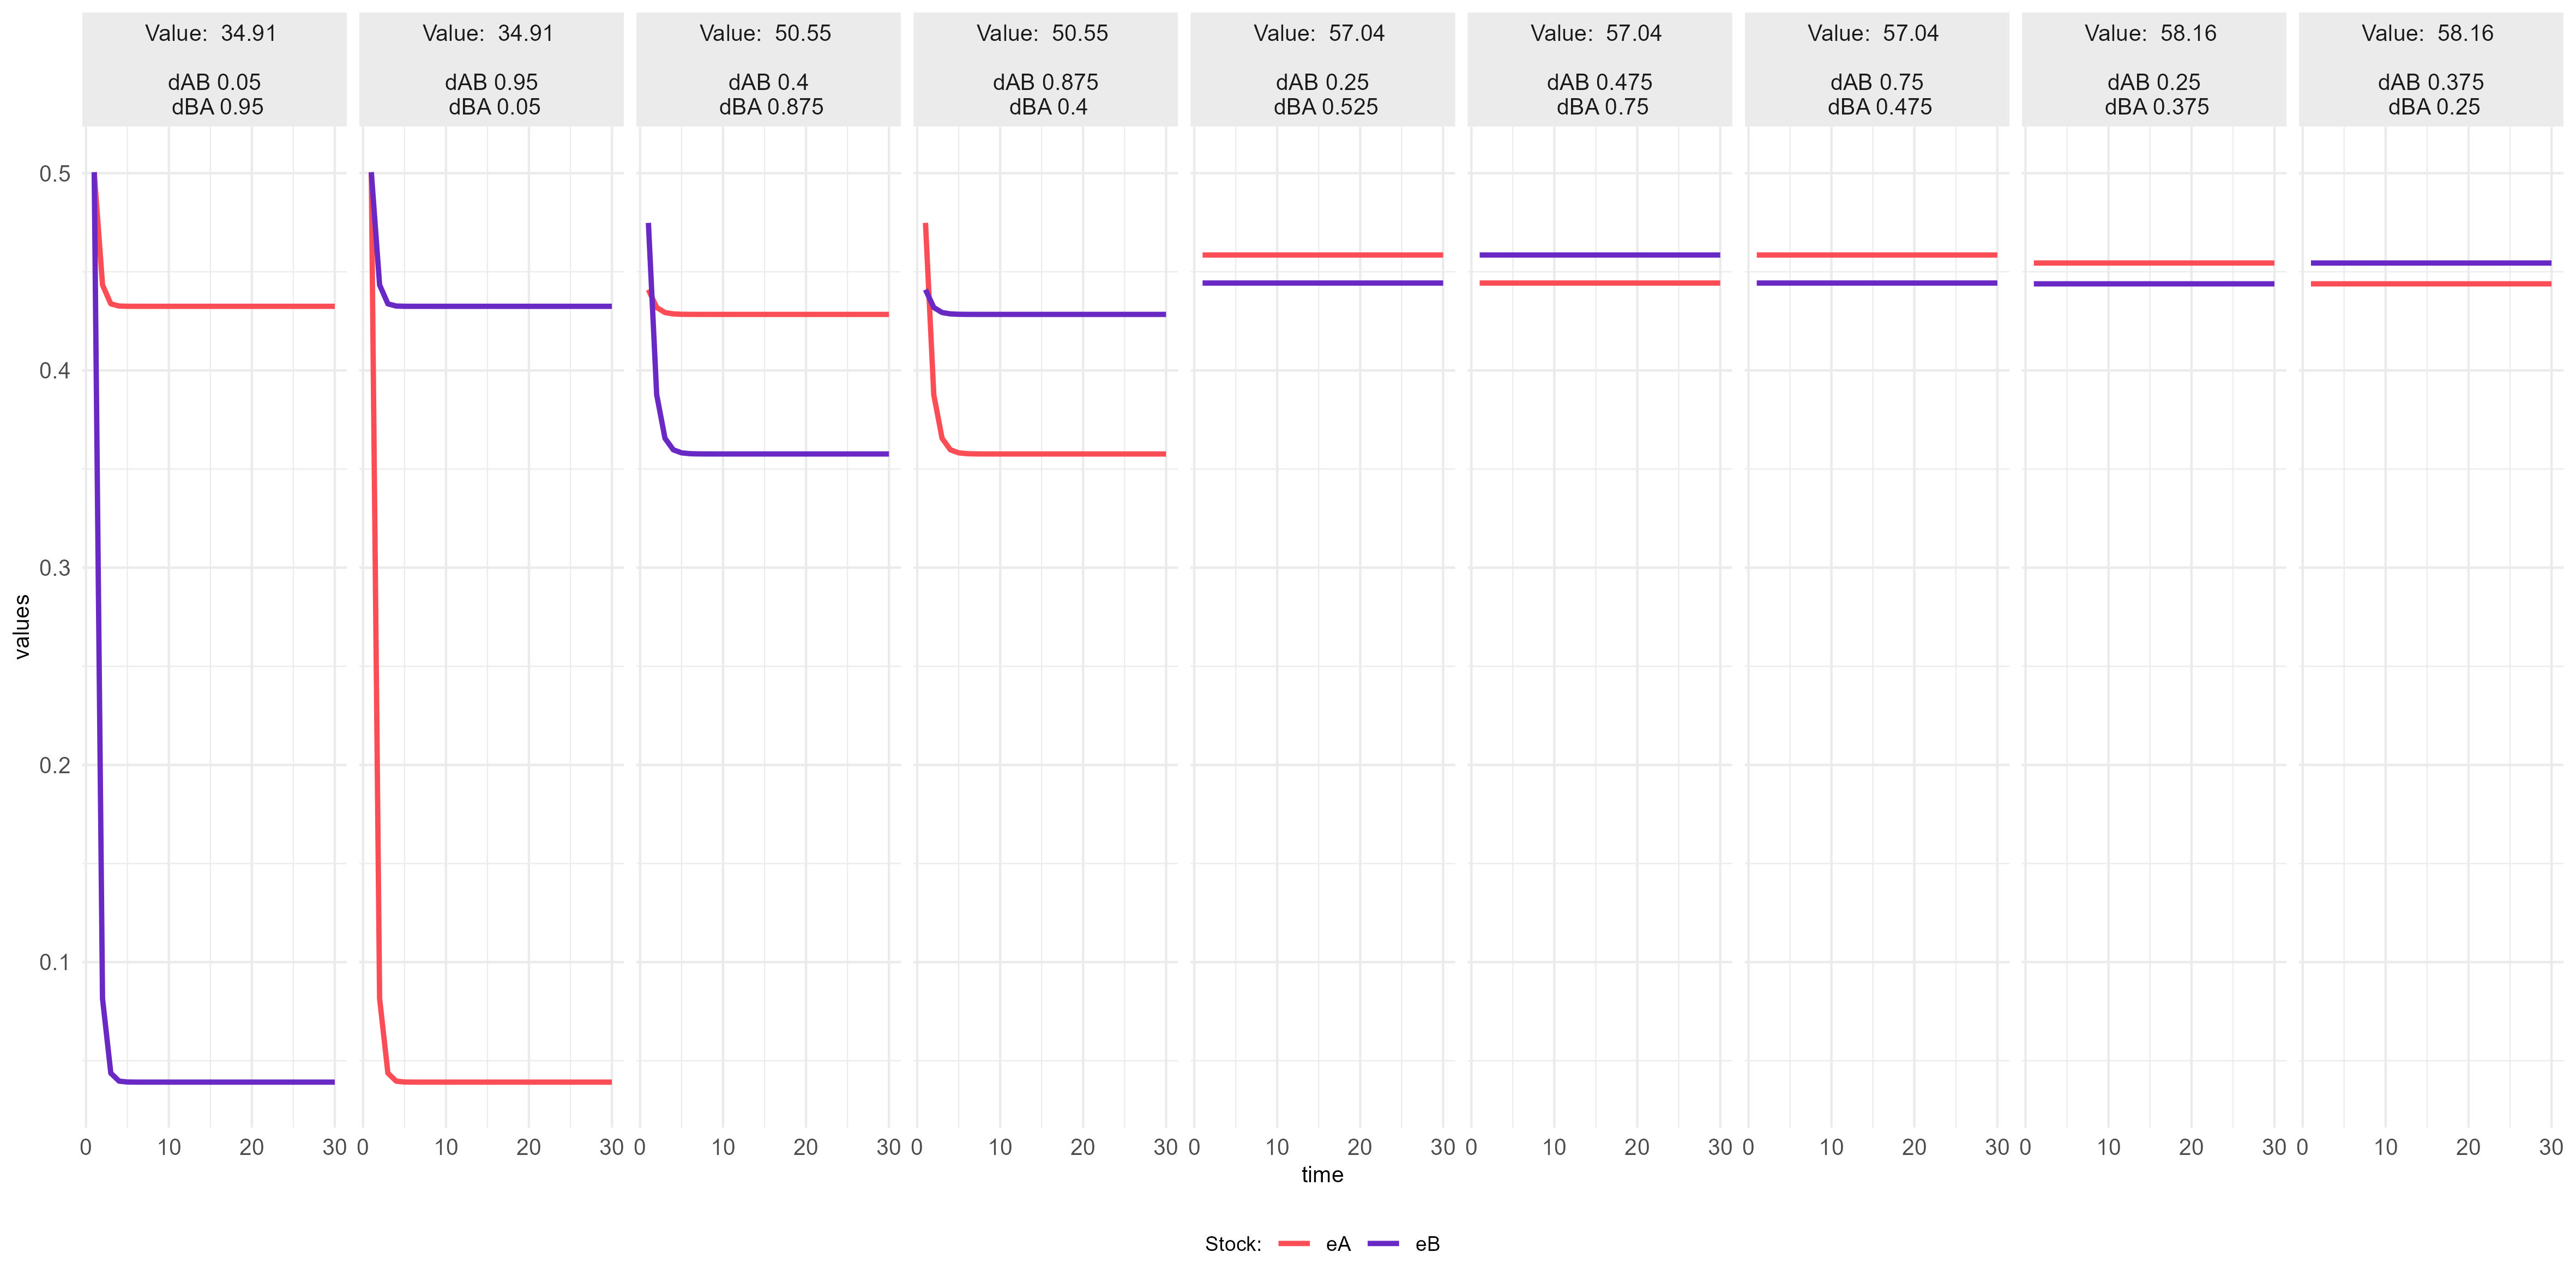
\includegraphics[width=\textwidth]{figures/fences/escapement_Baseline.jpg}
        \caption{Optimal stock and residual stock levels across patches for quartiles of the value function}
        \label{fig:figure1}
\end{figure}

Figure \ref{fig:escapement_derivative_interior} shows the variations in residual stock for interior and corner solutions. For low values of dispersal from $A$ to $B$, residual stock in $A$ decreases, but increases after $d_{AB}>.5$. Variations depend on the relative magnitude of $d_{AB}$ and $d_{BA}$, and display the non linear trends highlighted in proposition \ref{prop:escapement_variation}. Finally, figure \ref{fig:escapement_derivative_overall} shows the evolution of optimal residual stock, constrained by low stock levels in respective patches. 


\subsubsection{Value and connectivity}

The mechanisms highlighted above are illustrated in the surface map of the value function across $d_{AB}$ and $d_{BA}$. For sink-source dynamics (top right and bottom left corners), the dispersal patterns allow to control more of the population, resulting in lower population through time and lower damages. As dispersal patterns are more symmetric, the optimal intertemporal costs tend to increase. Ultimately, although the numerical values only serve an illustrative purpose, they show a stark result: if connectivity is manageable at limited costs, leveraging spatial arbitrage opportunities can increase welfare by almost 40\%. 

\begin{figure}[H]
	\centering
	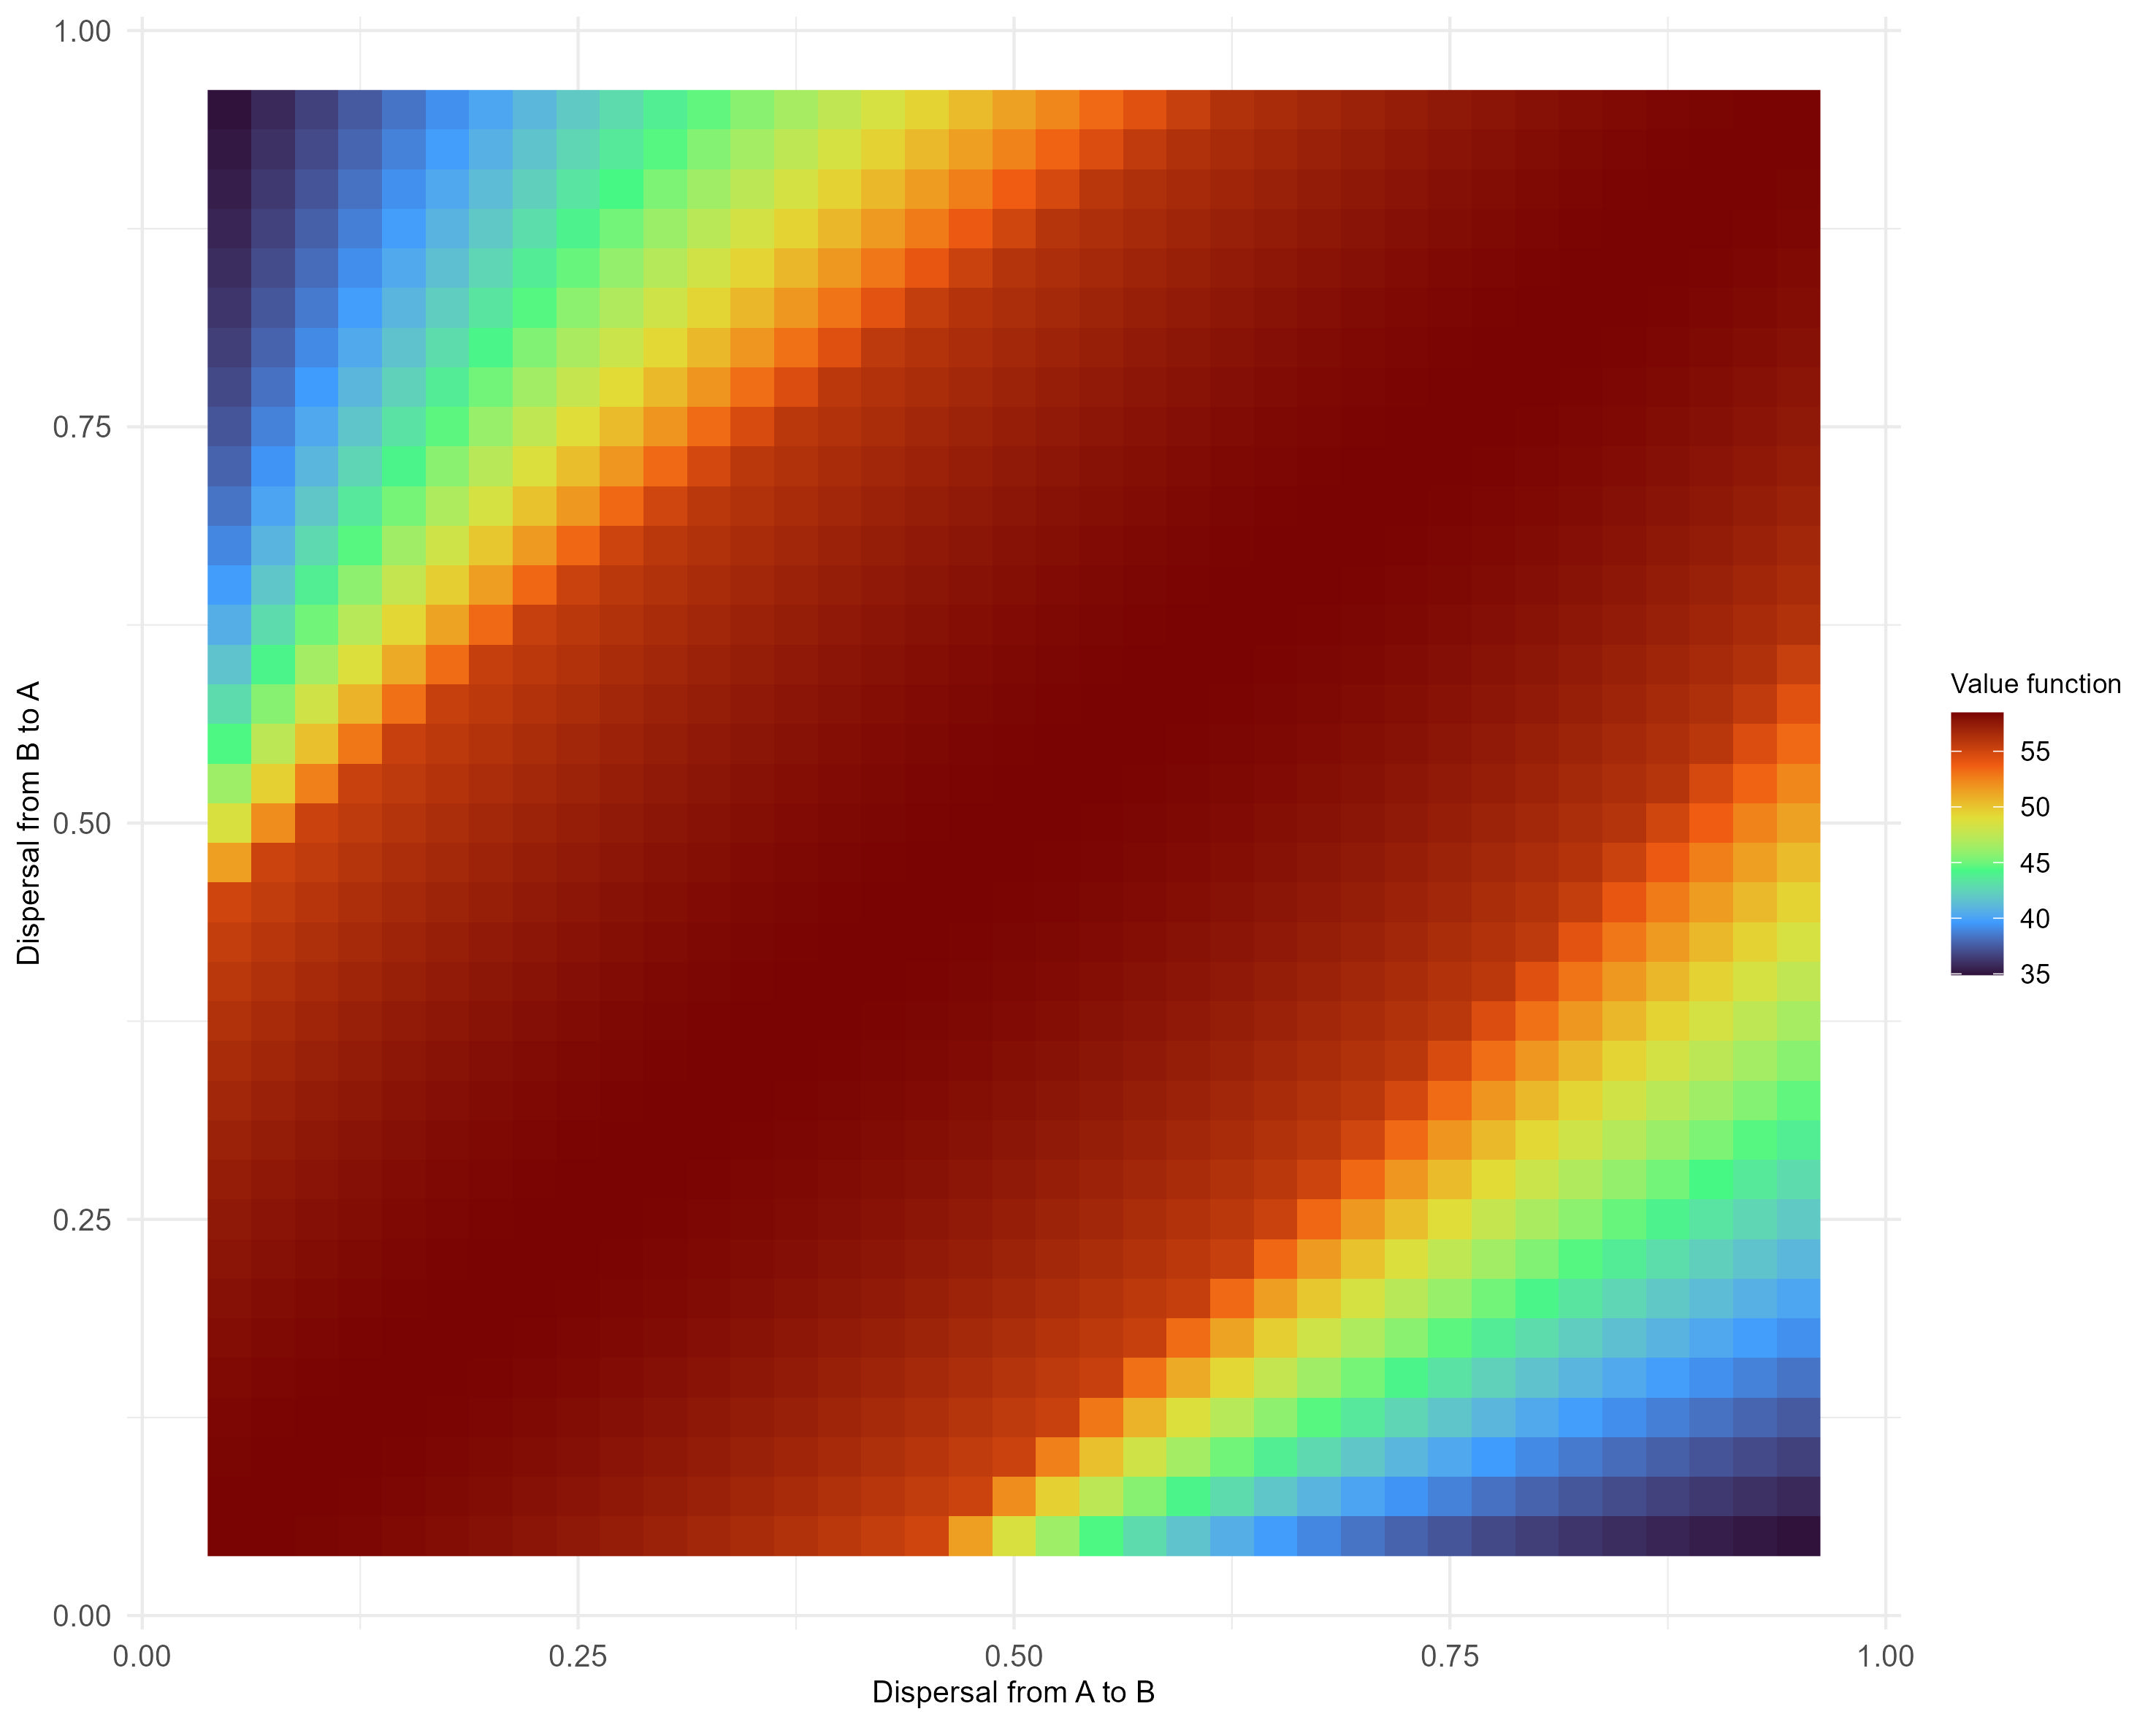
\includegraphics[width=.8\textwidth]{figures/fences/heat_map_values_Baseline.jpg}
	\caption{Intertemporal costs of mobile public bad depending on landscape connectivity patterns}
\end{figure}



\section{Introducing fences}
\subsection{Definition and properties}
\label{sec:subsection_fences_definition}
As there is value to manage connectivity, connectivity measures are likely being implemented, unless they are prohibitively costly. In this part of the model, dispersal rates between patches depends on directional fencing expenditures in both patches, with $d_{ijt+1} \equiv d_{ijt+1}(f_{it}, f_{it})$, where $f_{it}$ measures the amount of fencing in patch $i$ in direction of patch $j$, as a percentage rate of maximal fencing, such that $F=\{f_{it} + f_{it} \leq 2\}$.  The rate of inward dispersion of invasive species from $i$ to $j$, $d_{ijt+1}(f_{it},f_{it})$ decreases with $f_{jt}$. I call this the "exclusionary effect": fences keep nuisances out of $j$. When fencing in $i$ at $f_{it}$, the outward dispersion of invasive species from $i$ to $j$ decreases as well, as species get trapped in $i$. This effect is the "trap effect" : fences trap the nuisance in. However, in most cases of exclusionary fencing, the exclusionary effect dominates the trap effect, allowing for trapped animals to escape. Fencing reduces the inward dispersion from $i$ to $j$ at a decreasing rate, whether it is undertaken in patch $i$ or $j$. The rate of patch retention $d_{iit+1}$ is the remainder after dispersions from $i$ to $j$. When no fencing is undertaken, the dispersal rate remains at a rate determined by immutable environmental factors (landscape discontinuities, mountains, terrain ruggedness etc), such that $d_{ijt+1}(0,0) = m_{ij}$. When the maximal amount of fencing is undertaken, dispersal drops to $n_{ij}$. 
Dispersal rates are ultimately affected by immutable environmental factors (landscape discontinuities such as roads, rivers, moutains; altitude and terrain ruggedness etc).
\begin{equation}
\begin{aligned}
d_{ijt+1} : F \to [n_{ij},m_{ij}] \subset [0,1] \\
\underbrace{\frac{\partial d_{jit+1}}{\partial f_{it}}}_{\text{Exclusionary effect}} \leq \underbrace{\frac{\partial d_{ijt+1}}{\partial f_{it}}}_{\text{Trap effect}} \leq 0\\
 d_{ijt+1}(f_{it}, f_{it}) + d_{iit+1} =1
\end{aligned}
\label{eq:dispersal_with_fences}
\end{equation}
As such, fences have public good features: whether $A$ or $B$ fences, both the inbound and outbound dispersal are affected, while only pf them pays the price.

In practice, for numerical simulations, I adapt dispersal rates from metapopulation theory using a negative exponential dispersal kernel \citep{hanski_estimating_2000, MOILANEN2004533}. Fencing acts as increasing the distance between patches, and conversely, as reducing the mean dispersal distance of a species in a given patch : 
\begin{equation}
d_{ijt+1}(f_{it},f_{jt}) = \exp(-\theta( f_{jit} + \beta_i f_{ijt})\times (m_{ij} - n_{ij}) + n_{ij}
\end{equation}
Where $\theta$ is a scaling parameter, and $\beta_i$ measures the relative effect of fences in $i$ compared to fences in $j$ to reduce $d_{ijt+1}$. Figure \ref{fig:dispersal_illustration} illustrates dispersal between $A$ and $B$ with asymetric bounds to dispersal (i.e. $m_{ij} \neq m_{ji}$ and $n_{ij} \neq n_{ji}$). 

\begin{figure}[H]
	\centering
	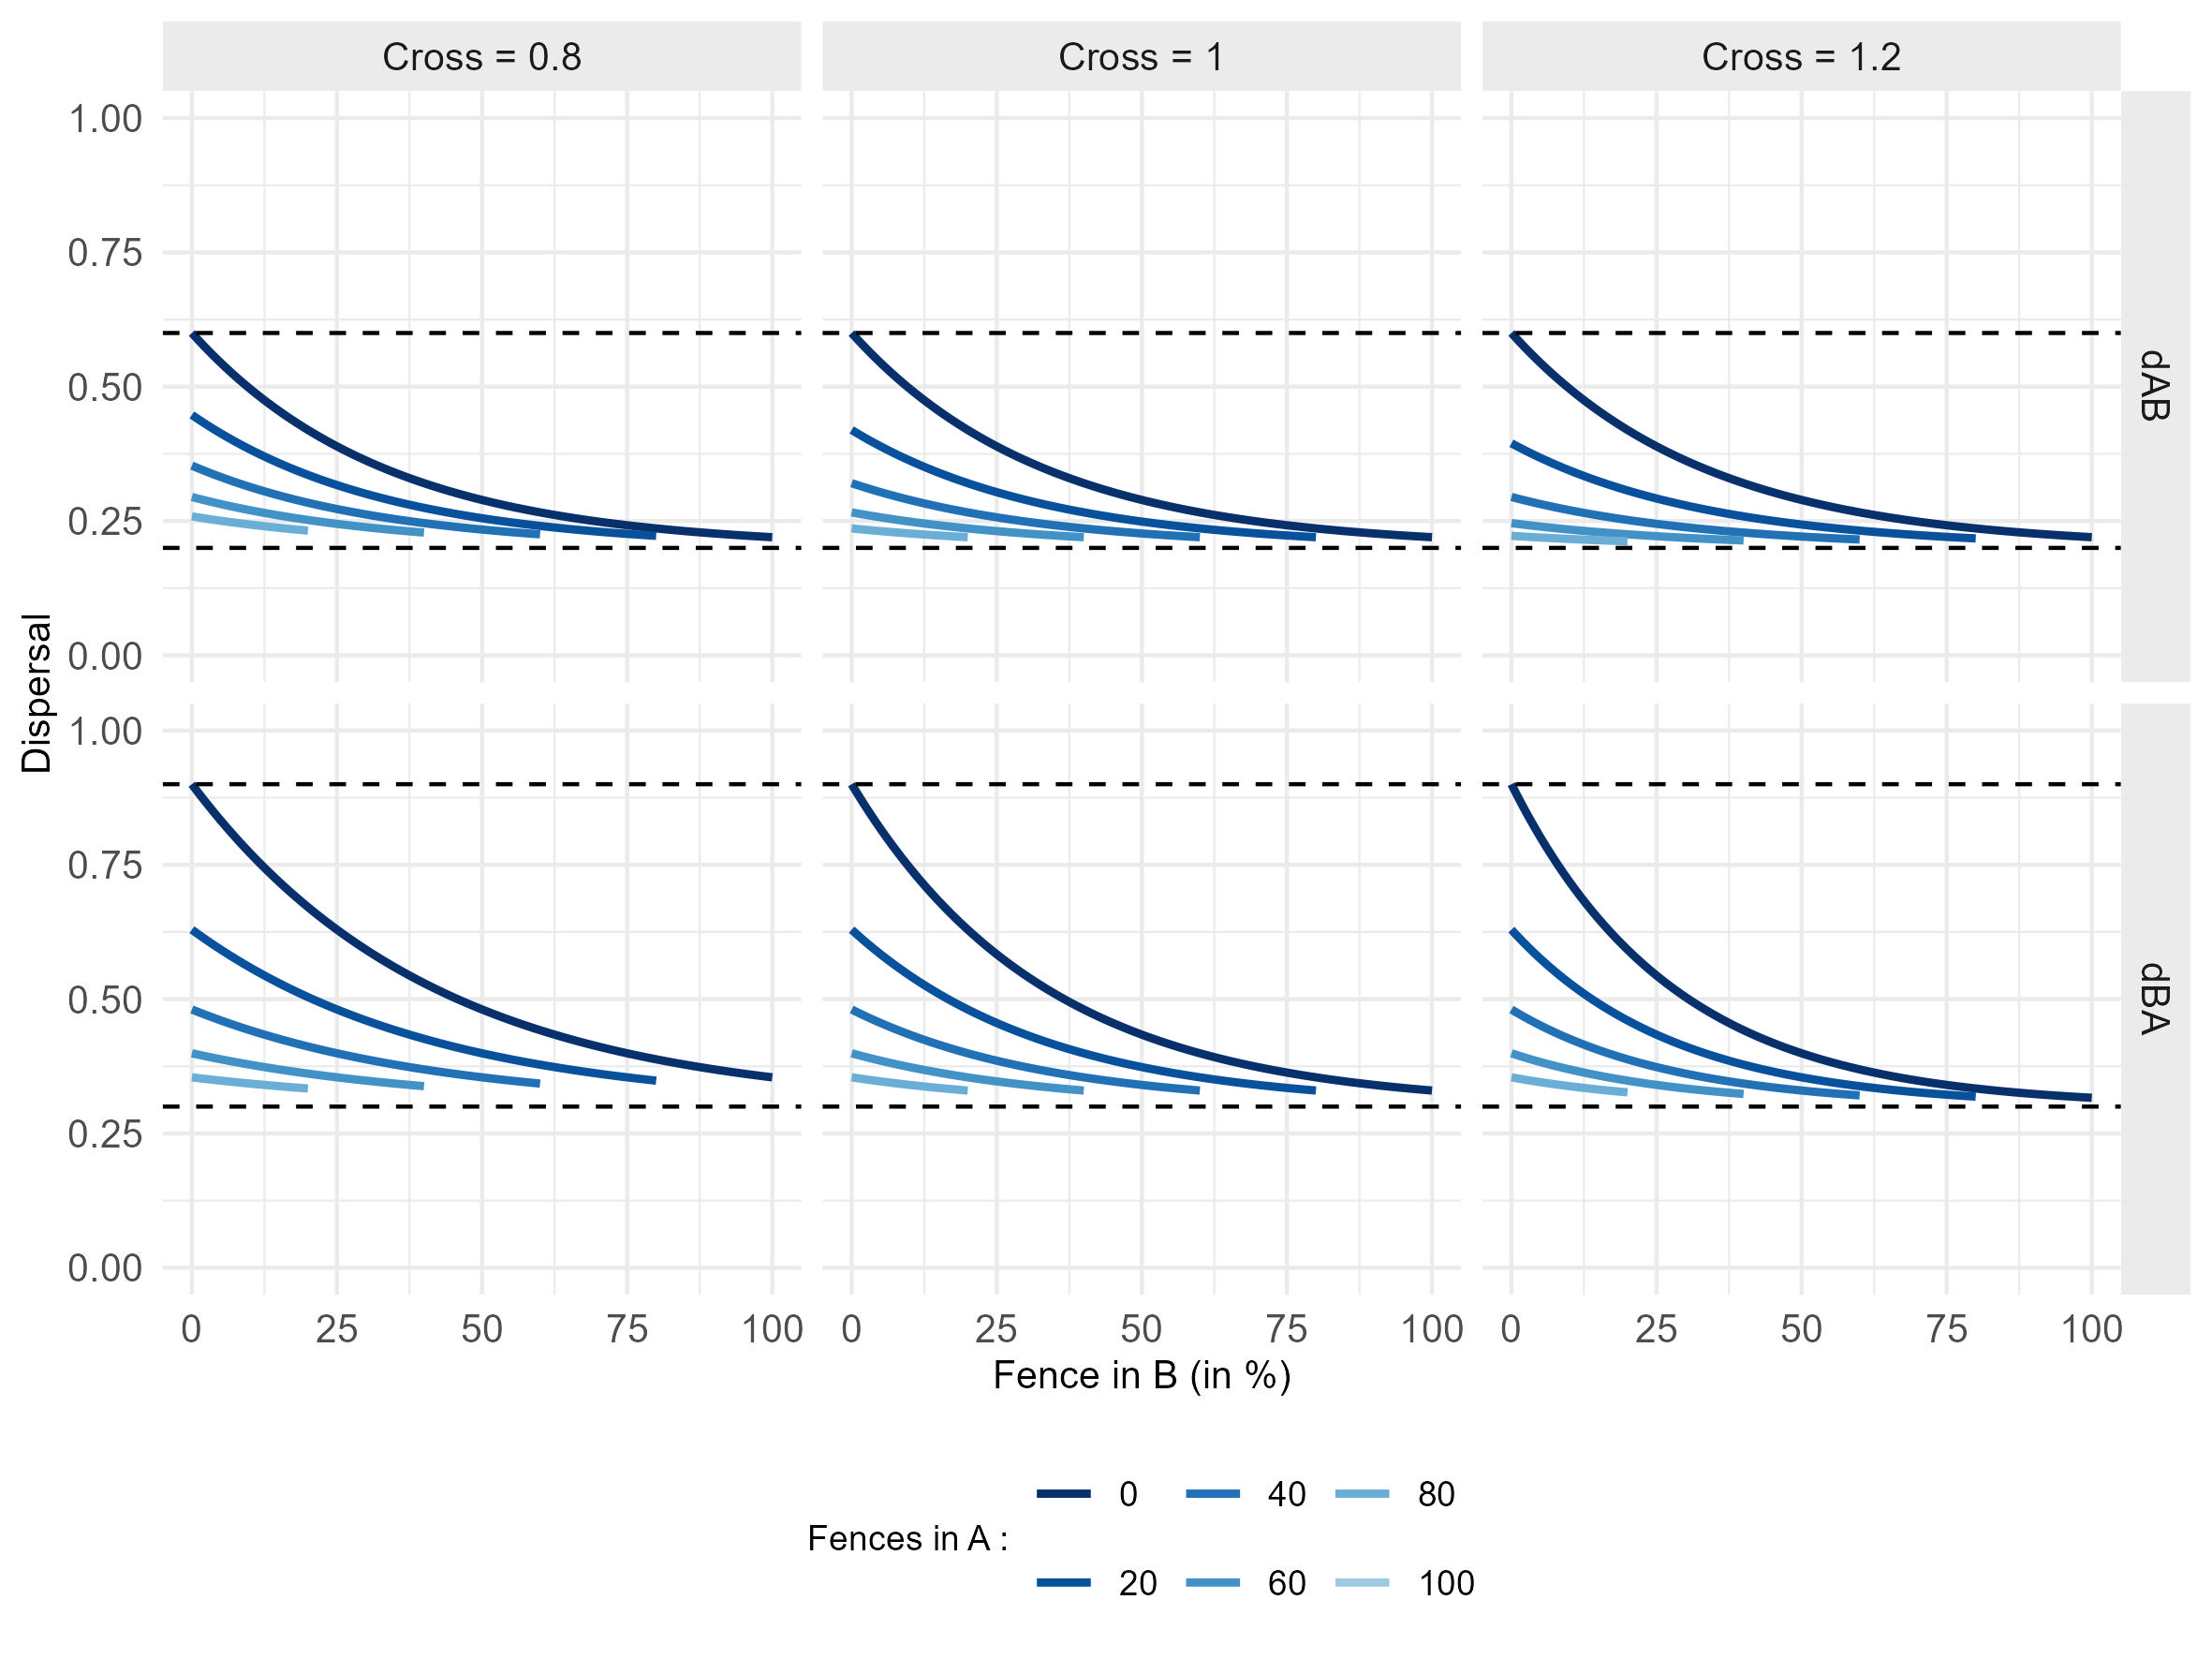
\includegraphics[width=.6\textwidth]{figures/fences/illustration_dispersal.jpg}
	\caption{Dispersal depending on fencing decision in $A$ and $B$ with asymetric bounds and cross efficiencies}
	\subcaption*{On the left panel, $\beta_A=.8$ describes a situation where the trap effect dominates, while on the right panel, $\beta_A = 1.2$ displays a situation where the exclusionary effect dominates}
	\label{fig:dispersal_illustration}
\end{figure}

Fences change dispersal in a specific way, as they only diminish connectivity \textit{between} patches, and increase self retention. In the case where patches have the same bounds to dispersal ($n_{AB} = n_{BA}$ and $m_{AB} = m_{BA}$), fencing is not in the interest of the social planner : 
dispersal remains symmetric, and the value function does not vary along the symmetry axis between $d_{AB}$ and $d_{BA}$. Indeed, when fencing retains as much population in as it does keep out, the net effect on the next period population is null. As fences come to a certain cost, it always outweighs inexistant benefits. However, when bounds to dispersal are asymmetric, fencing can have a positive effect on welfare. As dispersal is decreased to asymetric inferior bounds, the population stock across patches changes asymetrically as well. In doing so, one can leverage the spatial arbitrage opportunity associated with asymetric dispersal and non-homogenous nonlinear costs, as well as different marginal damages. 


\begin{figure}[htbp]
    \centering
    \begin{subfigure}{0.45\textwidth}
        \centering
        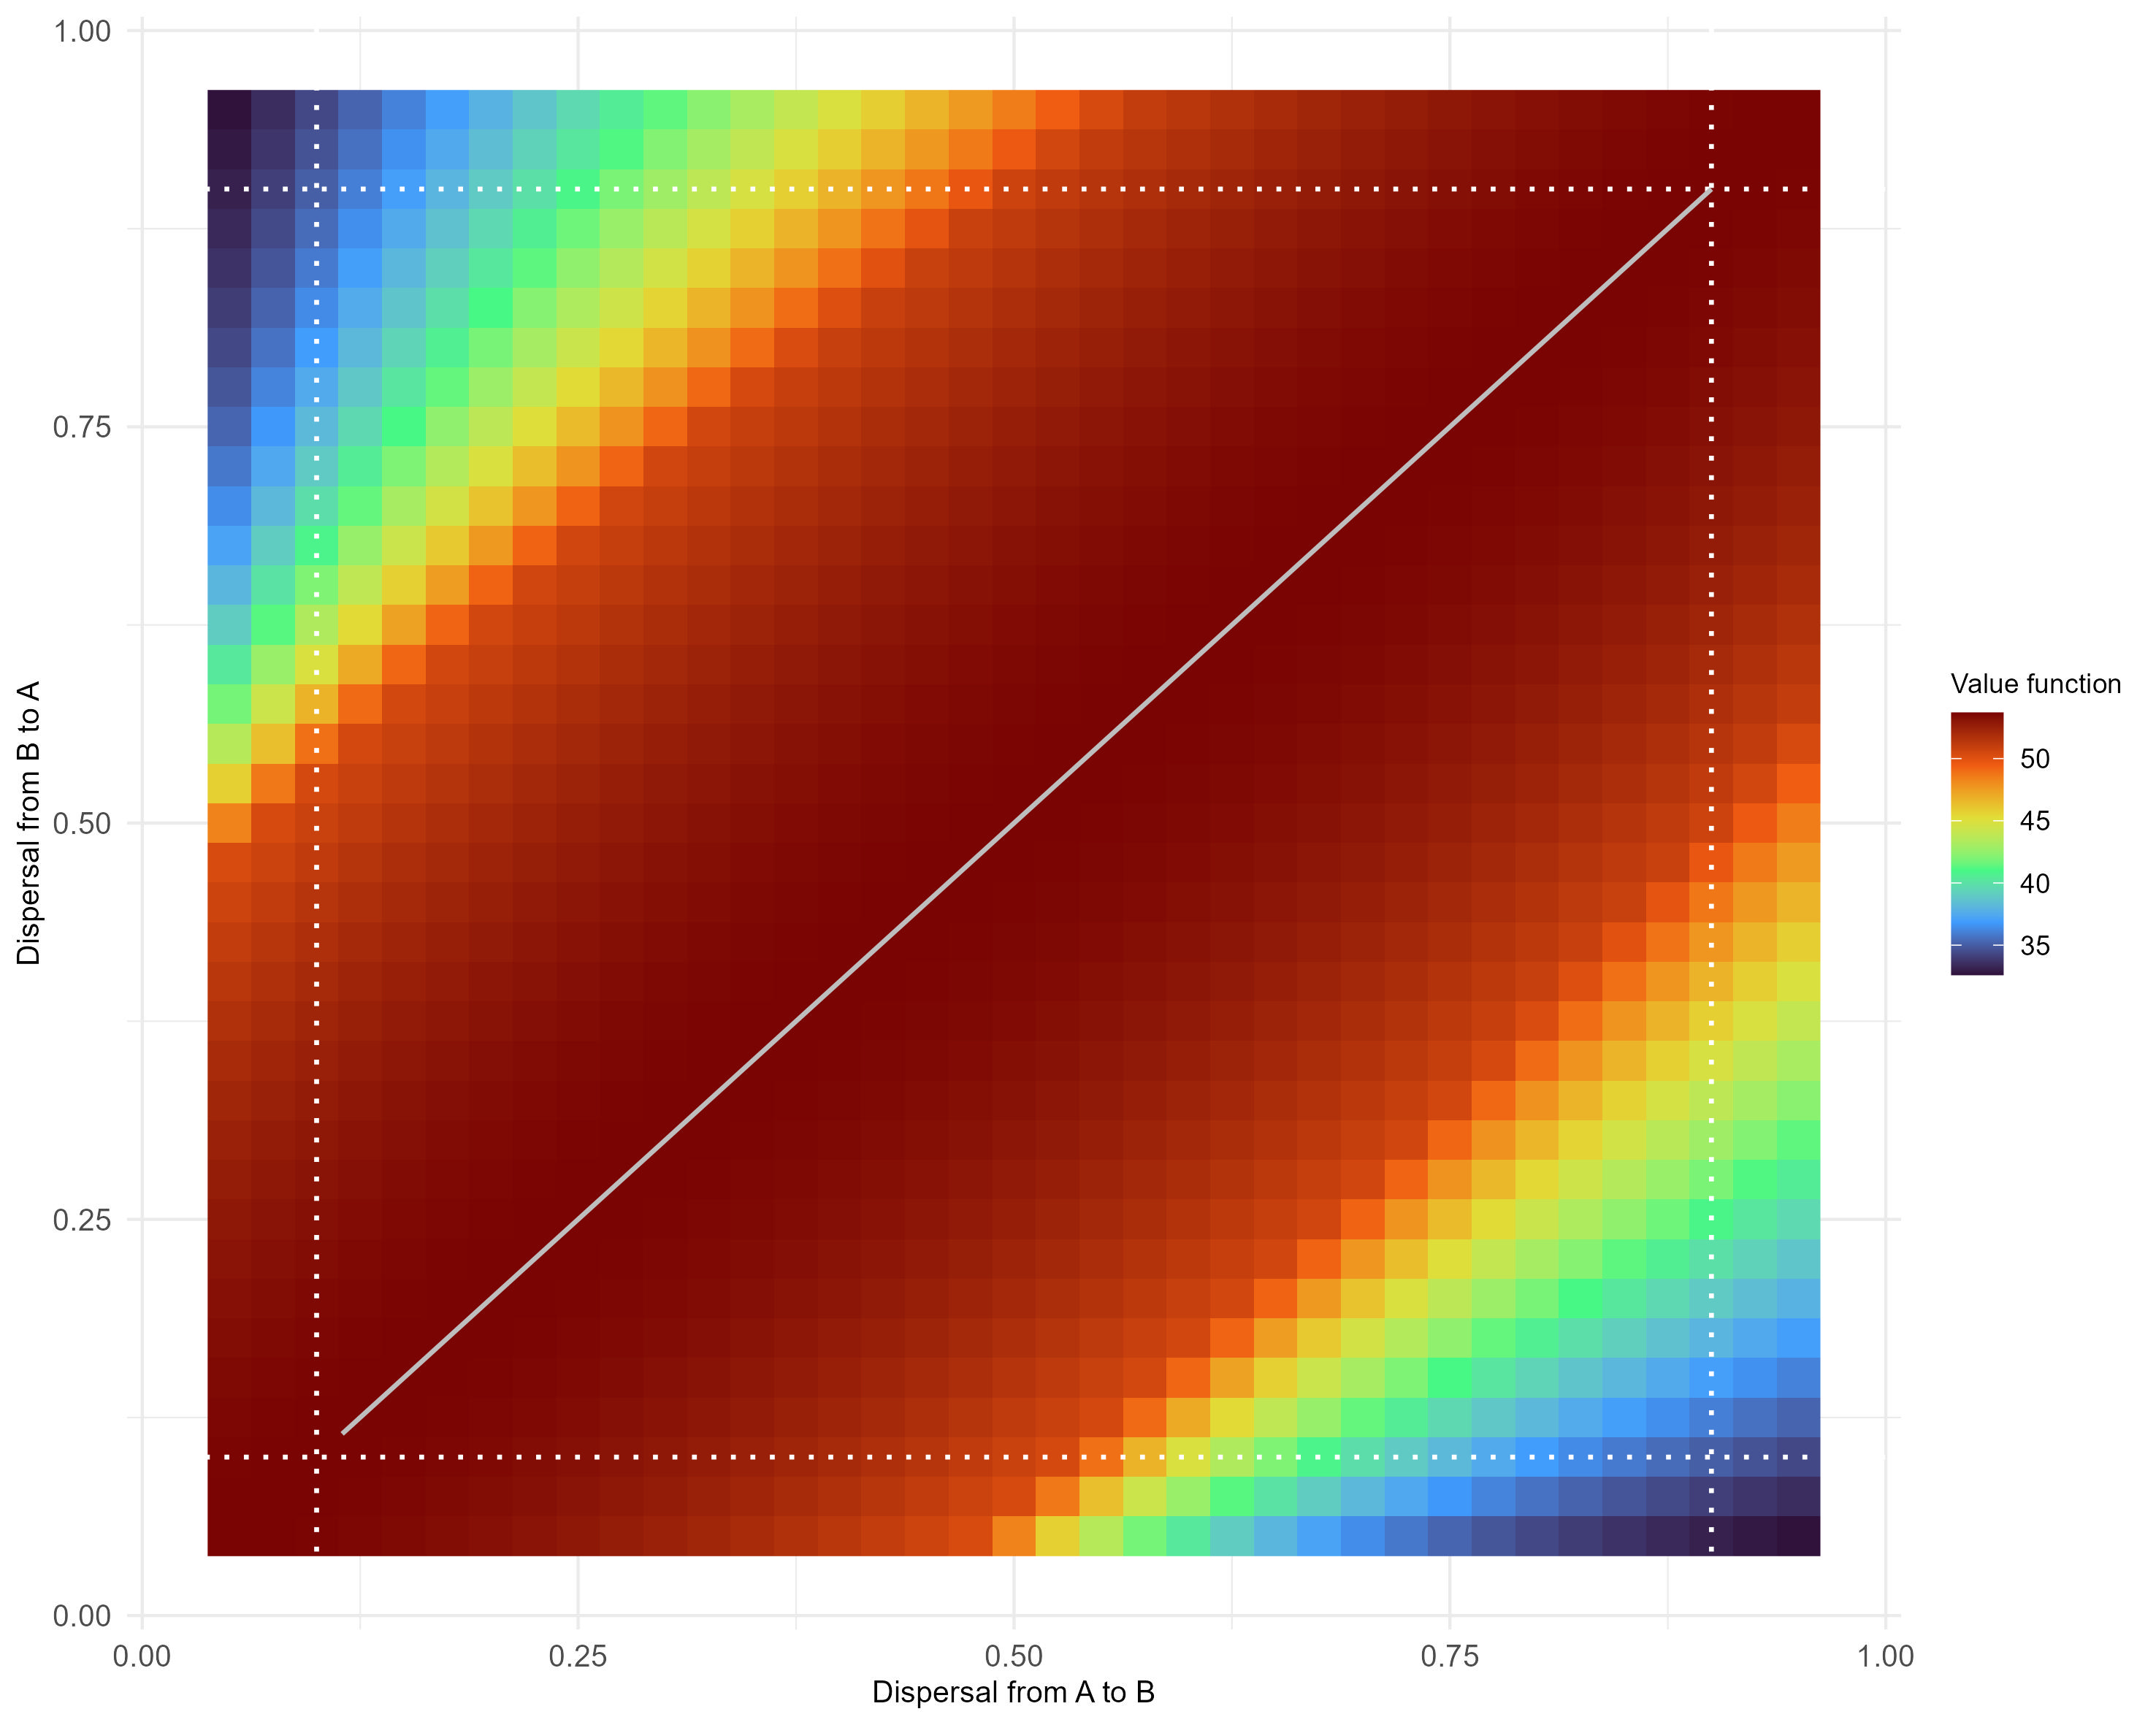
\includegraphics[width=\textwidth]{figures/fences/heatmap_with_symmetric_dispersal_large.jpg}
        \caption{Inefficient changes in connectivity with symmetric natural bounds}
        \label{fig:figure1}
    \end{subfigure}
    \hfill
    \begin{subfigure}{0.45\textwidth}
        \centering
        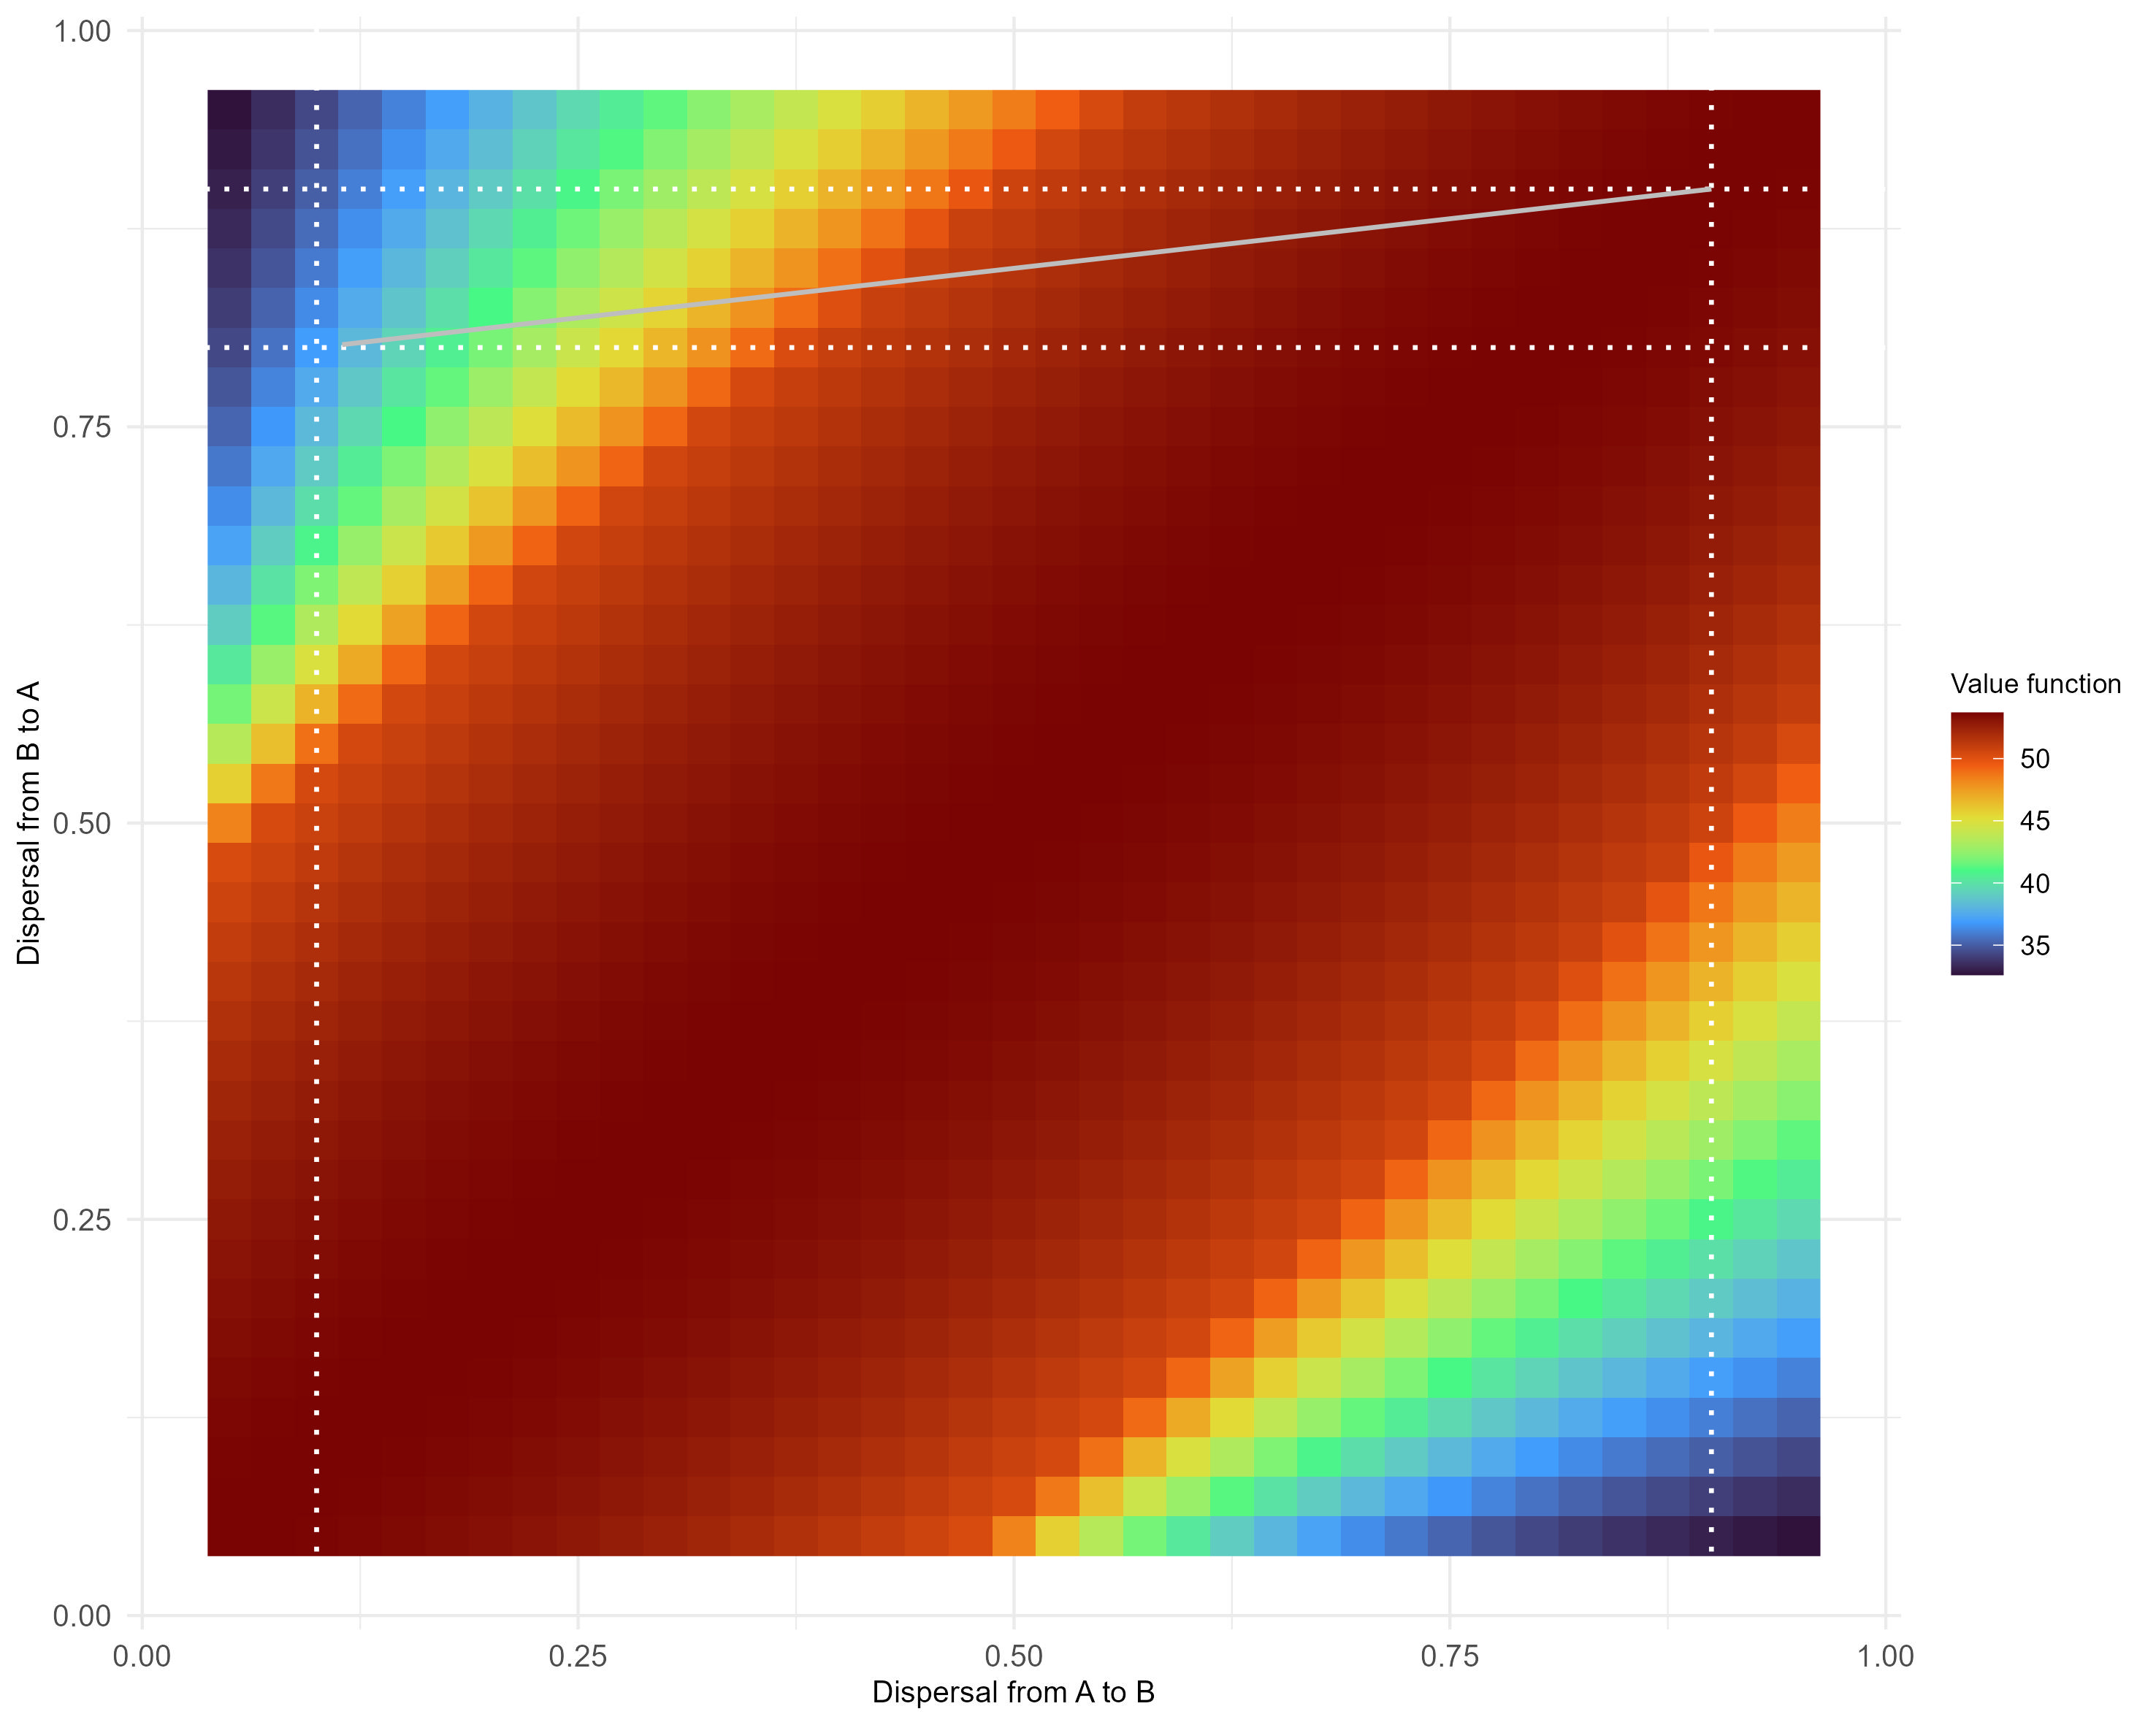
\includegraphics[width=\textwidth]{figures/fences/heatmap_with_asymmetric_dispersal.jpg}
        \caption{Efficient changes in connectivity with asymmetric natural bounds}
        \label{fig:figure2}
    \end{subfigure}
    \caption{Efficient and inefficient changes in landscape connectivity}
    \label{fig:overall}
\end{figure}

\subsection{Spatial ecology and economy with fences}

With fences, the spatial ecology of the problem is modified as follows, with $d_{ijt+1}(f_{it}, f_{it})$ defined as in equation \ref{eq:dispersal_with_fences}: 

\begin{align}
X_{it+1} &=  d_{jit+1}(f_{it}, f_{it}) g_j(e_{jt}) + \left(1 - d_{ijt+1}(f_{it}, f_{it})\right)g_i(e_{it}) \nonumber \\
& = g_i(e_{it}) + \left( d_{jit+1}(f_{it}, f_{it}) g_j(e_{jt}) - d_{ij}(f_{it}, f_{it}) g_i(e_{it}) \right)
\end{align}

Fences are expressed as a percentage of the maximal rate of fencing doable. Anecodtal evidence suggests that fencing costs increase in a convex way: marginally reducing the passage of species or viruses can be done at a low costs, while more efficient devices can reach large costs\footnote{Methods range from scent and taste-based repellents, that need to be reapplied frequently and cost 15-50\$ per gallon, to electric fencing (at 3-5\$ a foot), and landscape modifications such as gullies and dams (ranging from 500 to 5,000\$ per work), and finally, regular human presence. In the case of viruses, strategies range from wearing surgical masks to partial and complete lockdowns, with different economic costs. \cite{gollier2020cost, acemoglu_optimal_2021} analyze the costs of different lockdown strategies with multigroup SIR models, in the context of COVID 19. They focus on age-specific disease spread rates, which is akin to considering spatially differentiated spread rates. They show that efficient, targeted lockdown strategies are paramount as their costs are convex.}. For the sake of simplicity, I nonetheless restrict the analysis to linear costs, such that the current payoff is modified. The total cost in each patch $i$ and period $t$ is : 
\begin{equation}
C_i(e_{it}, X_{it}, f_{it}^1, ..., f_{it}) = \int_{e_{it}}^{X_{it}}c_i(s)ds + \int_{0}^{e_{it}}k_i(s)ds  +  \kappa_i f_{it}
\end{equation}


















%\section{A spatially disconnected world}
%
%
%\subsection{Optimal fencing and controling}
%\label{sec:optimal_management}
%Assume a sole owner has to manage patches $1$ to $N$. She can decide how much to control in each patch, as well as to what degree patches are connected to minimize the total cost of the public bad, through time.  Her aim is to equalize the dynamic marginal costs of pest through space and time. 
%
%Her objective is to minimize the present value of aggregate costs across patches over time:
%
%\textbf{write the optimization program}
%
%The Bellman equation is :
%\begin{equation}
%V(X_{1t}, ..., X_{Nt}) = \min_{\forall i \{e_{it}, \{f_{it}\}_{j\neq i}\}} \sum_{i = 1}^N C_i(e_{it}, X_{it}, f_{it}^1, ..., f_{it}) + \delta V(X_{1-t+1}, ... X_{Nt+1})
%\label{eq:bellman}
%\end{equation}

%As a benchmark, we characterize the optimal control of the species in each patch, if each patch is isolated and dispersal cannot be managed (or at prohibitive costs) by the social planner (e.g.$\forall i,j$, $m_{ij}=n_{ij}=0$, thus $d_{ijt+1}(f_{it}, f_{it}) = 0$). As in \cite{costello_private_2017}, the first order conditions for an interior solution are : 

%\begin{proposition}
%\label{proposition:benchmark_no_space}
%If $\forall i,j$, $m_{ij}=n_{ij}=0$, then, $\forall i,j$ and $\forall t$ : 
%	\begin{align}
%		f_{it} &= 0\\
%	\end{align}
%	And : 
%	\begin{align}
%	\bar{e}_{it} > 0 &\iff k_i(\bar{e}_{it}) = c_i(\bar{e}_{it}) -  \delta g_i'(\bar{e}_{it})c_i(X_{it+1})\\
%	\bar{e}_{it} = 0 &\iff k_i(0) - c_i(0) \delta g_i'(0)c_i(0)>0
%		\label{eq:control_no_space}
%	\end{align}
%	
%\end{proposition}
%
%This result is expressed in \cite{costello_private_2017} in proposition 5 and 6. In a spatially disconnected world, the sole-owner controls the efficient amount in each patch. For an interior solution, the current marginal damage must equal the marginal cost of control, net of the future costs of control imposed by controling one more unit of the bad. However, if the marginal damages are sufficiently low, or the dynamic costs expected to rise sharply, then the optimal solution is eradication. As such, in a disconnected world, local eradication and interior solutions can coexist. Additionally, as connectivity cannot be managed, the marginal benefits of any fence are null, hence there is no fence. 
%Proposition \ref{proposition:benchmark_no_space} establishes that fact. 

%\subsection{Non cooperative equilibrium}

%\textbf{Establish the correspondence in the decentralized case. }
%In this case, each patch owner optimally controls the patch specific population, accounting for a dynamic stock effect : as the population is treated at a lower level, marginal growth is important and lowers the future cost of effort. 

\section{A world with endogenous connectivity and population}

\subsection{Socially optimal management: conditions for interior solutions}

When dispersal can be managed (i.e. $n_{AB}\neq m_{AB}$ and/or $n_{BA}\neq m_{AB}$), the sole owner decides both the levels of fencing and residual stock. Proposition \ref{proposition:optimal_sole_owner} establishes the conditions under which both interior fencing and residual stock exist:

\begin{proposition}
\label{proposition:optimal_sole_owner}
Interior optimal residual stock in each patch $i$ is such that : 
\begin{equation}
k_i(e_{it}) = c_i(e_{it}) - \delta g'_i(e_{it})\left[c_i(X_{it+1}) + d_{ijt+1}(f_{it}, f_{it})c_j(X_{jt+1}) - c_i(X_{it+1})) \right]
\label{eq:optimal_harvest}
\end{equation}

And optimal fencing in patch $i$ towards patch $j$ is : 
\begin{equation}
\kappa_i = \delta\left(\frac{\partial d_{ij+1}}{\partial f_{it}} g_i(e_{it}) - \frac{\partial d_{jit+1}}{\partial f_{it}}g_j(e_{jt})\right) \big(c_i(X_{it+1}) - c_j(X_{jt+1})\big)
\label{eq:optimal_fencing}
\end{equation}
Additionally, interior fencing and control are state-independent i.e. solutions do not depend on $\mathbf{X}_t$ (see proof in appendix \ref{appendix:proof_stock_independence_foc}).
\end{proposition}

 The optimal residual stock in patch $i$ is such that the current marginal damage caused by letting the marginal unit matches the corresponding control cost, mitigated by the discounted global cost effect, as in \cite{costello_private_2017} (refered to as the \textit{dynamic marginal cost effect}). When a marginal unit of bad is controlled, marginal damage $k_i(e_{it})$ are not incurred in patch $i$. This marginal damage has to equal the current period cost of controling $c_i(e_{it})$, and the discounted next period cost. A marginal unit of bad will grow according to $g_i'(e_{it})$, and disperse through space. A portion $d_{iit+1} = 1 - \sum_{j\neq i}d_{ijt+1}(f_{it}, f_{it})$ remains in the patch (and sets the marginal cost of control at $c_i(X_{it+1})$, while a fraction goes in each connected patch $j$, incurring a decrease in marginal control costs of $c_j(X_{jt+1})$. The extent of control thus depends on the current marginal damages and costs, and the spatial dynamic component. If dispersal to neighbors is \textit{naturally} large, and the marginal cost of control tends to be lower in these patches, residual stock increases, leveraging a spatial arbitrage opportunity.

Interior fencing is a novel result. In a given patch, the sole owner fences such that the current marginal cost of fencing equals the discounted marginal benefits of fencing. These benefits emerge from the use of a spatial arbitrage opportunity. Positive fencing occurs in $i$ if the \textit{exclusionary} effect of fencing (i.e. the marginal population that remains in $j$ following an increase in fencing in $i$) outweighs the \textit{trap} effect (i.e. the marginal population that remains in $i$ following an increase in fencing in $i$), and the marginal cost of control are larger in $i$ than in $j$. Positive fencing in $i$ can also emerge if the \textit{trap} effect dominates the \textit{exclusionary}, but control costs are larger in $j$ than in $i$. To further characterize the optimal management, I restrict the analysis to the case of constant marginal costs of control. In the next subsections, I disentangle the effects of the trap and exclusion effects with constant marginal costs of control.


\subsubsection{No fencing in the absence of spatial arbitrage opportunity}

The spatial arbitrage opportunity arises from the difference in control costs across space and for different stock levels. In that case, the absence of control cost heterogeneity implies no fencing : redirecting the resource flow has no interest, since there is no additional cost reduction to be expected. Although patches are connected, there is no heterogeneity to leverage. As a consequence, the optimal control rule is independent of dispersal. 
 In this case, the discounted future cost of controlling the increased stock in patch $i$ equal the current costs net of damages. Moreover, the optimal control does not depend on spatial dispersal, as the cost of control are homogenous, and depends only on patch specific characteristics. In this specific homogeneous linear case, the equilibrium collapses to the disconnected optimal control strategy defined in proposition \ref{proposition:homogeneous_cost}.

\begin{proposition}
\label{proposition:homogeneous_cost}
With linear homogeneous control costs (e.g. $\forall i$, $c_i(s) = c$), or no spatial dispersal (i.e. $d_{ii} = 0$ and $d_{jj}=0$), optimal management consists in no fencing $\forall i, j$, $f_{it} = 0$ and optimal residual stock is implicitly defined by:
$$
		c \delta g_i'(e_{it}) = c - k_i(e_{it}) 
$$
See proof in appendix \ref{appendix:proof_absence_fencing}
\end{proposition} 


\subsubsection{Optimal management with heterogeneous costs and exclusionary fencing}
\label{sec:optimal_exclusionary}

Assume control costs are heterogeneous, such that $c_A> c_B$. In this case, there is a potential to levy a spatial arbitrage opportunity : if the stock were more directed towards patch $B$, larger levels of control could be undertaken with the same budget (or equivalently, the same amount of aggregate control could be undertaken at a lower cost). 
In this example, I assume fencing only has an exclusionary effect. In real life, exclusionary fencing is a common practice in conservation. For example, the Kilauea Point National Wildlife Refuge in Hawaii has implemented a predator exclusion fence to protect native seebirds from mammalian predatiors\footnote{The 11,200 foot fence protects 168 hectares of wildlfe habitat and even includes underground skirt and curved hood to avoid climbing over or digging under, see \url{https://www.fws.gov/story/2023-08/pacifics-largest-predator-exclusion-fence}}. I focus on the case where exclusionary fences allow the population of predators to escape\footnote{In this case, the fencing technology can be seen as akin to an electrical resistance}.\\
In patch $A$, if fencing only has an \textit{exclusionary effect} and no \textit{trap} effect, fencing keeps the stock from $B$ out, while allowing the stock from $A$ to escape. Upon fencing, the sole owner gains clear marginal benefits, as the stock that used to flow from $B$ to $A$ no longer does, and the stock can still flow from $A$ to $B$, reducing the total cost. In this case,  the sole owner has an interest in reshaping how the stock moves through space, and thus, to reshape the spatial externality, such that resources flow to patch $B$.\\

\begin{proposition}
\label{prop:exclusion_optimal}
With heterogeneous, constant marginal cost of fencing such that $c_A>c_B$, $[n_{ij},m_{ij}] \subset ]0,1[$ and fencing only displays an exclusionary effect i.e. : 
\begin{align*}
& d_{ijt+1}(f_{it},f_{jt}) = d_{ijt+1}(f_{jt})\\
& \frac{\partial d_{ijt+1}}{\partial f_{jt}}<0
\end{align*}
The optimal allocation is : 

\begin{align}
\kappa_A &= \delta(c_A - c_B)\left|\frac{\partial d_{BAt+1}}{\partial f_{At}}(f_{At}^*, 0) \right|\\
f_{Bt}& = 0\\
k(e_{At}) &= c_A - \delta g_A'(e_{At})\large(c_A (1-d_{ABt+1}(0)) + c_B d_{ABt+1}(0))\large)\\
%
k(e_{Bt}) &= c_B - \delta g_B'(e_{Bt})\large(c_B (1-d_{BAt+1}(f_{At}^*)) + c_A d_{BAt+1}(f_{At}^*)\large)
\end{align}
\end{proposition}
Proposition \ref{prop:exclusion_optimal} shows that when spatial arbitrage opportunities are not exhaustable, the sole owner fences only in $A$ to avoid inward dispersal from $B$, while it does not change how much $B$ receives inward dispersion, as any dispersion from $A$ to $B$ is welfare improving. The response of optimal residual stock to changes in dispersal depends on the second order conditions of the problem\footnote{As a matter of fact : 
\begin{equation}
\frac{\partial e_{Bt}}{\partial f_{At}} = \frac{\kappa_A}{SOC_B}\delta g'(e_{it})
\end{equation}
Where $SOC_B = k_B'(e_{Bt}) + \delta g''_B(e_{Bt})((1 - d_{BAt+1}(f_{At}^*))c_{B} + d_{BAt+1}(f_{At}^*)c_A)$ is the second order condition of the problem with respect to $e_{Bt}$. As I do not fully analyze the second order conditions, it is impossible to substantiate claims further. However, notice that is negative when the increase in the marginal damage is lower than the increase in dynamic costs, and positive otherwise. As conditions for a global minimum differ with multivariate objective functions, this is a possibility to investigate further}.

%Eradication occurs in patch $A$ if 
%\begin{equation}
%k_A(0) - c_A + \delta g_A'(0)[(1-d_{ABt+1}(f_{At}^*,0)) c_A + d_{ABt+1}(f_{At}^*,0)c_B) >0
%\end{equation}
%And : 
%\begin{align*}
%\forall t>1, \text{ }e_{At} &= 0 \\
%k_B(e_{Bt}) &= c_B - \delta g_B'(e_{Bt})\large(c_B (1-d_{BAt+1}(0,f_{At}^*)) + c_A d_{BAt+1}(f_{At}^*,0)\large)
%\end{align*}
%Additionally, if fencing is free and connectivity can integrally be managed (i.e. $n_{ij} = 0$ and $m_{ij}=1$ $\forall i \in \{A, B\}$), damages are homogeneous ($k_A() = k_B() = k()$) then : 
%\begin{align*}
%f_{At} &= 1 \\
%f_{Bt} &= 0 \\
%\Rightarrow & d_{ABt+1} = 1 \text{ and } d_{BA} = 0\\
%\forall t>1, \text{ }e_{At} &= 0 \\
%k_B(e_{Bt}) &= c_B - \delta g_B'(e_{Bt})c_B
%\end{align*}
%\end{proposition}
%\subsubsection{Free fencing} 
Assume now that fencing only has a trap effect. For example, small scale fencing has long been used in the US to manage feral pigs populations, where animals get entrapped, but more can come in\footnote{see \url{https://www.aphis.usda.gov/sites/default/files/managing-feral-pigs.pdf}}. In patch $A$, if fencing only has a \textit{trap effect} and no \textit{exclusionary} effect, fences keep the stock inside of $A$, while they do not reduce the inward dispersion from patch $B$. As costs of control are smaller in $B$ than in $A$, a sole owner would benefit from keeping the population in $B$ where it is cheaper to control, and let the population from $A$ get trapped in $B$. The mechanism described here is \textit{in fine} symmetrical to the \textit{exclusionary} case, but fences are located in $B$.

%The sole owner can choose management to equate returns across space. When there is a spatial dependence, and connectivity is fixed by natural parameters, patches with high marginal costs of control, control less than in the no-dependence case. Symmetrically, patches with low marginal costs of control control less when they are not connected, as they can benefit from the dynamic marginal cost effect with population inflow from other patches. When the extent of connectivity can be managed (e.g. $n_{ij}>0$ and $0< m_{ij}\leq 1$), fencing arises in high control cost patches, and is kept at the minimal level in low control cost patches. In doing so, escapement decreases in high cost patches, and increases in low cost patches. 

%\begin{proposition}
%	If fences are free and only have an exclusionary effect, fences and control are substitutes
%	\\
%	see proof in appendix \ref{sec:appendix_proof7}.
%\end{proposition}


\subsubsection{Optimal management when fencing displays exclusionary and trap effects}

In most cases, fences has a both an \textit{exclusionary} and \textit{trap} effect, e.g. fencing reduces the inward dispersion from other patches to a given patch $A$, and reduces the outward population dispersion from patch $A$ to other patches. Following equation \ref{eq:optimal_fencing}, two effects are at play. First, fencing still results from a spatial arbitrage opportunity, from the spatial heterogeneity in marginal control costs. Second, the interplay between the \textit{exclusionary} effect and the \textit{trap} effect is key for fencing to be welfare improving, and biological productivity becomes important to decide where to locate the fences. In the case of patch $A$, optimal fencing arises if more of the pest population is kept out than in, while optimal fencing in $B$ arises if more of the population is kept in than out.

\begin{proposition}
\label{proposition:optimal_fencing_both_effects}
	When fencing has both an exclusionary effect and trap effect, with (i) heterogeneous costs of control, (ii) homogeneous cost of fencing, (iii) identical dispersal and (iv) the exclusionary effect dominates he trap effect, fencing occurs in patch $i$ if: 
	\begin{enumerate}
	\item $c_i>c_j$ and the exclusionary effect dominates the trap effect for some values of $e_{it}, e_{jt}, f_{it}$ : 
	\begin{equation}
	\frac{\kappa}{c_i - c_j} + \left|\frac{\partial d_{ijt+1}}{\partial f_{it}}\right|g_i(e_{it}) < \left|\frac{\partial d_{jit+1}}{\partial f_{it}}\right|g_j(e_{jt})
	\label{eq:optimal_fencing_both_effects_ci}
	\end{equation}
	\item $c_i<c_j$ and the trap effect dominates the exclusionary effect for some values of $e_{it}, e_{jt}, f_{it}$: 
		\begin{equation}
	\frac{\kappa}{c_j - c_i} + \left|\frac{\partial d_{ijt+1}}{\partial f_{it}}\right|g_i(e_{it}) > \left|\frac{\partial d_{jit+1}}{\partial f_{it}}\right|g_j(e_{jt})
	\end{equation}
	\item If fencing occurs in patch $i$, it does not occur in patch $j$
	\end{enumerate}
	
See proof in appendix \ref{appendix:heterogenous_cost_trap_exclusion}
%\textbf{Characterize the corresponding optimal levels}
\end{proposition}

Proposition \ref{proposition:optimal_fencing_both_effects} states that fencing in patches $A$ depends on control cost, biological productivity heterogeneity, and the relative effects of fencing. When fences keep as much out as they keep in, biological productivity must be such that benefits from fencing still emerge due to initially large population levels and heterogeneous constant marginal costs of control. Contrary to the case of variable marginal control costs, heterogeneity in the bounds of dipsersal, and thus on the effects of fences, does not provide any spatial arbitrage opportunity alone. \\
With heterogeneous costs of control, this result shows that fencing is optimal (at least temporarily and partially) to isolate a patch with a large growth : this result concurs with \cite{Wilen2012} who find isolation to be a welfare improving strategy (in a different modeling system, with spatially explicit cellular automata). In real life, temporary quarantine is applied at small scales (for example within a cattle) and larger scales (such as the country scale during epidemics such as the foot and mouth disease in 2001 in the UK).  When fences play more of an exclusionary than trap effect, a naive argument would call for fencing in $A$ as long as the rate at which fencing decreases inward dispersion from $B$ is larger than the rate at which fencing increases self retention in $B$. However, population levels matter. Indeed, if population growth is sufficiently high in $A$, the self retained population in $A$ may be very large, even though the rate of self retention increases at a slower pace than the rate of inward dispersion from $B$ decreases.  Finally, with homogeneous growth, fencing in $A$ is incompatible with fencing in $B$.\\

To conclude, in the presence of spatial heterogeneity in control costs, optimal management leverages a spatial arbitrage opportunity. Dispersal rates are modified to take advantage and redirect pest populations where they are least costly. However, if in a patch, biological growth and control costs are larger than in the other patch, fencing may not be optimal, as the retained population causes additional burden as it tries to avoid more population inward dispersion from the cheap, low growth patch.

% Proposition \ref{proposition:biological_heterogeneity_optimal} establishes the effect of biological heterogeneity for management. 

%\begin{proposition}
%\label{proposition:biological_heterogeneity_optimal}
%	Establish previous claim : if biological productivity in patch $i$ is such that 
%	\begin{equation*}
%	\min_s g_i(s) > \max_s \frac{\frac{\partial d_{jit+1}}{\partial f_{it}}}{\frac{\partial d_{ijt+1}}{\partial f_{it}}}g_j(s)
%	\end{equation*}
%the spatial cost heterogeneity is not enough to warrant fencing, as biological productivity is so large that the trap effect always dominates. \\
%Further characterize that with the correlation between cost function and growth. 
%\end{proposition}

%Finally, when control costs are stock dependent, the spatial arbitrage opportunity can be exhausted when either costs of control are equalized across patches, or when the exclusionary effect equals the trap effect. In the former case, the result on optimal escapement remains unclear, while in the second case, it has been characterized to replicate the disconnected equilibrium. 

\subsection{Non cooperative equilibrium}

I now turn to the analysis of the non cooperative equilibrium, where each patch owner determines their optimal level of control and fences in each period. Two effects are at play. First, the spatial externality is not internalized in a non cooperative equilibrium : the costs borne by neighboring patches are not internalized, hence resulting in under control, as highlighted in \cite{costello_private_2017}. Second, the equilibrium provision of fences will depend on their properties, whether they are only exclusionary or also display a trap effect. Fences allow to resolve the spatial dependency on other players, i.e. they solve the spatial externality. However, they also feature public good properties, as fencing in $A$ not only reduces the outward dispersion from $B$ to $A$, but also the inward dispersion from $A$ to $B$.
Each patch owner in $A$ and $B$ aims to minimize the present value cost subject to choices in residual stock and fences: 
\begin{equation}
V_{it}(\mathbf{X}_t) = \min_{e_{it},f_{it}}\left(\int_{0}^{e_{it}}k_i(s)ds+\int_{e_{it}}^{X_{it}} + \kappa_i f_{it} + \delta V_{it+1}(\mathbf{X}_{t+1}) \right)
\end{equation}

In what follows, I use Markov Perfect Nash Equilibrium as a solution concept. The residual stock and fencing rules from an MPNE if given information about the population levels in $t$, they are optimal rules for subsequent periods. 
In line with the previous part, I assume linear costs of control. In the case of an interior equilibrium, residual stock and fencing by each player is characterized by : 
\begin{proposition}
The interior equilibrium is characterized by residual stock and fencing levels in patch $i$ given by : 
\begin{align}
k_i(\bar{e}_{it}) & = c_i\big( 1 - \delta g_i'(\bar{e}_{it})(1 - d_{ijt+1}(\bar{f}_{jt},\bar{f}_{it}))\big)\\
\kappa_i 	& = \delta c_i\left(\frac{\partial d_{ijt+1}}{\partial \bar{f}_{it}}g_i(\bar{e}_{it}) - \frac{\partial d_{jit+1}}{\partial \bar{f}_{it}}g_j(\bar{e}_{jt}) \right)
\end{align}
See proof in appendix \ref{appendix:interior_mpne}
\end{proposition}

In this case, each landowner does not internalize the costs she's causing the other, hence this results in under residual stock in the case of interior solutions. Second, the fencing strategy of each owner only depends on their costs, and not on the cost differential. The optimal fencing strategy is determined such that the marginal cost of fencing ($\kappa_i$) equals the discounted marginal benefits of fencing i.e. the cost of the marginal change in net dispersion flow following a change in fencing in $A$.\\
To gain further intuition, assume a fully homogeneous world : control costs and fencing costs are homogeneous ($c_A = c_B = c$ and $\kappa_A = \kappa_B = \kappa$), the effect of fencing on the outward dispersal flow are identical, and the effect of fencing on the inward dispersal flow are identical (i.e. $\frac{\partial d_{ABt+1}}{\partial f_{At}} = \frac{\partial d_{BAt+1}}{\partial f_{Bt}}$ and $\frac{\partial d_{ABt+1}}{\partial f_{Bt}} =\frac{\partial d_{BAt+1}}{\partial f_{At}}$).

\subsubsection{Homogeneous costs, growth and damages.}

To gain intuition, assume fencing only displays an exclusionary effect i.e. $\frac{\partial d_{ijt+1}}{\partial f_{it}}=0$. This example is in many ways simplifying (especially as marginal costs of control are assumed linear), but captures essential intuition. For example, during the COVID pandemic, from March to June 2020, the European Union issued \href{https://www.consilium.europa.eu/media/47592/st_9208_2020_init_en.pdf}{temporary restrictions} on non-essential travel \textit{into} the EU, along with other states such as the \href{https://www.dhs.gov/archive/news/2020/10/19/fact-sheet-dhs-measures-border-limit-further-spread-coronavirus}{United States}.
In this case, a race to the bottom in terms of connectivity arises, as fences do not feature public good properties. As each player builds more fences, it increases the share of pest remaining in the neighboring patch. In doing so, it increases the dynamic costs and damages inflicted on the neighbor. Every player has an interest in fencing up to the point where the the cost of increasing fencing equals the avoided cost from decreasing the inward dispersion flow. No player has an interest to deviate from this strategy: if player $A$ fences below the individual marginally efficient level, player $B$ does not decrease her fences, and more population flows from $B$ to $A$, resulting in lower costs and damages for $B$. Hence, the equilibrium is a situation where both players overfence compared to the optimum  and undercontrols. \\
In the limiting case where dispersal can be completely shut down (for example, if the marginal cost of fencing $\kappa$ is low compared to damages) such that $d_{ijt+1} = d_{jit+1} = 0$, individual residual stock is optimal, as shown in proposition \ref{proposition:homogeneous_cost}. However, the fencing level is suboptimal. 

\begin{proposition}
With (i) constant homogeneous marginal cost of control, (ii) homogeneous costs of fencing, (iii) homogeneous growth and marginal damage and (iv) homogeneous exclusionary fencing, the non cooperative equilibrium is : 
\begin{align}
k(\bar{e}_{it}) &= c(1 - \delta g'(\bar{e}_{it})(1 - d_{ijt+1}(\bar{f}_{jt}))\\
\kappa & = c \left|\frac{\partial d}{\partial f_i}\right| g_j(\bar{e}_{jt})
\end{align}
Under direct application of the first order conditions
\end{proposition}

Now, assume fencing displays a both exclusionary and trap effects. Assume the exclusionary effect dominates the trap effect, such that $\left|\frac{\partial d_{ijt+1}}{\partial f_{jt}}\right| > \left|\frac{\partial d_{ijt+1}}{\partial f_{it}}\right|$ and $\frac{\partial d_{ijt+1}}{\partial fjt} = \beta_j(f_{jt})\frac{\partial d_{ijt+1}}{\partial f_{it}}$ with $\beta_j(f_{jt})\geq 1$. In the case of constant marginal costs of control, \cite{costello_private_2017} show that the equilibrium residual stock in each patch increases with inward and outward dispersal rates. As the exclusionary effect dominates, increases in fencing in each patch decrease inward dispersal more than outward dispersal. Additionally, residual stocks decreases. Hence, each player has an incentive to increase fencing to decrease the inward dispersal flow, and no interest in deviating, as the exclusionary effect dominates : upon deviation, residual stock in the neighboring patch increases, and the inward dispersal share increases, causing additional costs and damages.
In the case of interior solutions, the non cooperative equilibrium results in suboptimal fencing, as fencing is undertaken in two patches. As a result, the interior non-cooperative equilibrium is inefficient. 

\begin{proposition}
When the exclusionary effect of fencing always dominates the trap effect, the decentralized equilibrium is given by : 
\begin{align}
k(\bar{e}_{it}) &= c(1 - \delta g'(\bar{e}_{it})(1 - d_{ij}(\bar{f}_{jt}))\\
\kappa_i  & = \delta c_i\left|\frac{\partial d_{ijt+1}}{\partial f_{it}}\right|(\beta_i(\bar{f}_{it})g_j(\bar{e}_{jt}) - g_i(\bar{e}_{it}))
\end{align}
Hence,  $\bar{f}_{it}>0$, $\bar{f}_{jt}>0$ and $\bar{e}_{it}\neq e^*_{it}$
\end{proposition}

If the exclusionary effect and the trap effect are identical and homogeneous across patches, in the decentralized equilibrium, no fencing is undertaken, as it reduces the individual welfare : upon fencing, each player incurs cost $\kappa$ while not changing the inbound or outbound rate of dispersal. In this case, the equilibrium is identical to the equilibrium extensively analyzed in \citep{costello_private_2017}.


\section{Discussion and conclusion}

In this article, I show that connectivity patterns play an important part in the intertemporal costs and damages associated with spatially distributed bads, with variable marginal costs of control. When dispersal patterns change, the optimal residual population in each patch has non-monotonous responses, as variable marginal costs of control may increase disportionately for low stock values. On the other hand, even at low marginal control costs, large increases in inward dispersal flows may cause large increases in control costs. In the end, changes in dispersal have ambiguous effects, and patterns closer to source-sink relationships are more cost efficient. \\
Second, I introduce fences, that modify the patterns of spatial connectivity. If control costs are homogeneous, or dispersal is prohibitively costly to change, there is no interest in modifying dispersal, as there is no spatial arbitrage opportunity to leverage. In the case of cost heterogeneity and homogeneous biological productivity, optimal connectivity management redirects the bads towards where they are cheapest managed. However, with heterogeneous growth, or initial population, optimal connectivity management changes connectivity patterns only if costs and growth are inversely correlated through space : in the case of large growth and costs, fencing may not be optimal, as the cost burdens can be spread through space. I then turn to the study of non-cooperative equilibria, with constant marginal costs of control. I show that in the case of exclusionary fencing, the equilibrium results in suboptimal connectivity degradation, although it fosters large levels of control in each patch, and solves the tragedy of the commons. However, in doing so, spatial arbitrage opportunities are left untapped. 

The comparison between the optimal and non cooperative equilibria rests on several simplifications. First, the analysis is built on the case of interior solutions, and little care is yet devoted to the analysis of corner solutions. As eradication is favored with larger spatial independence, the analysis of the switch towards eradication in both the optimal and decentralized equilibrium lacks to fully compare the two, and is left for future work. The existing comparison nonetheless provide important insights on the management of population and connectivity, in a spatially explicit framework. \\
Second, the analysis rests on the assumption of constant marginal costs of control, while the original analysis of this model rests on the hypothesis of stock dependent marginal costs of control. In doing so, I avoided to consider the elasticity of control costs, which guide the evolution of optimal and decentralized residual stocks and fences, in a non monotonous fashion. While variable costs refine the analysis, the conceptual insights based on spatial arbitrage opportunity remain, in the absence of cost heterogeneity among patches.  \\
Third, this model does not consider density dependence in dispersal patterns, which allows interior solutions to be state independent. I chose to focus on the interplay of human decisions on connectivity and population management and disentangle their relative effects rather than focusing on the evolution of population alone. I believe this structure of migration may be useful for situations where densities in each patch remain small, such that agglomeration effects of the population are too low to force migration outside of patches. 

Additionally, the model developed here is not fully characterized. Overall, the effects of heterogeneity have not yet been integrated in the framework. Examples of analysis that relate the correlation of the distributions of control costs and biological productivities show that heterogeneity among patches plays an important role in the optimal management of populations and connectivity, in the case of interior solutions. This effect may be bolstered in the case of (partially corner solutions), to study how fencing promotes eradication, under what conditions does temporary fencing foster long term benefits. 

I have identified four avenues of future research. First, the current two patch structure leaves global connectivity concerns difficult to study. Indeed, as this article is concerned with endogenous ecological-economic network formation, the small scale of the analysis precludes me from deriving interesting network scale results \citep{bode_using_2008}, especially in the case of original invasion and optimal response of neighboring patches. . This opens the second research avenues, which involves characterizing the effects of heterogeneity on optimal network formation and population management, as well as on the decentralized equilibrium, contributing to the literature on network formation games \citep{griffith_continuous_2022} in the context of renewable resources. As the effects of heterogeneity matter on small and large scale, I plan on analyzing the policy mix that can be implemented to reconcile the optimum and the non cooperative equilibrium. 
Intuition show that while implementing the first best policy mix, which reshuffles resources to the most cost effective patch is always best, it is not always achievable in practice. Analyzing the second best allocation is important. When a policy maker can only choose 1 instrument, i.e. either population or connectivity control, it is unclear which should be favored, and how the choice of this instrument depends on the heterogeneity of the costs, damages, growth and initial populations across the landscape. The fourth research avenue implies factoring in risk in the ecological dynamics : invasions are stochastics, and risk aversion may increase a tendency towards fencing. It is unclear how the optimal allocation of resources accounts for this effect. 

\section*{Acknowledgements}
I am grateful to Christopher Costello, Lauriane Mouysset, Martin Quaas, Laurent Lamy, Romain Fillon, Dimitri Goldztejn and Alexandre Adrian at Platt Vineyard as well as to seminar participants at the Parisian PhD Seminar in Environmental Economics (PPSEE), at the FAERE Doctoral Workshop (USMB, Annecy), at the Biodiversity Economics Research Group Seminar at iDiv (Leipzig), and at CIRED for their valuable comments.


\clearpage
\counterwithout{figure}{section}
\counterwithout{table}{section}
\setcounter{figure}{0}
\setcounter{table}{0}
\setcounter{equation}{0}
\numberwithin{equation}{section}
\renewcommand{\thesection}{\Alph{section}}
\renewcommand{\thesubsection}{\Alph{subsection}}
\renewcommand{\thefigure}{2.\Alph{figure}}
\renewcommand{\thetable}{2.\Alph{table}}



\phantomsection
\addcontentsline{toc}{section}{Appendix}
\section*{Appendix}  % Use section* for no numbering
\renewcommand\theequation{A.\arabic{equation}} % Prefix equation numbers with A
\setcounter{equation}{0}
\label{sec:appendix}

\subsection{Model timing}

\begin{figure}[H]
  \centering
  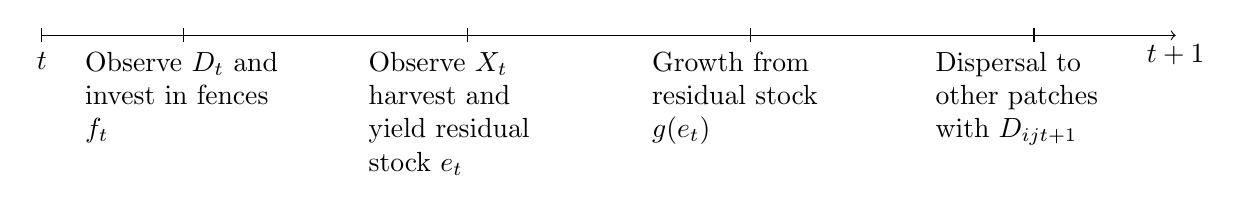
\begin{tikzpicture}[scale = .9]
    % Draw the arrow
    \draw[->] (0,0) -- (16,0) node[anchor=north] {$t+1$};
    % Draw ticks and labels
    \draw (0, .1)--(0,-.1) node[anchor = north]{$t$};
    \draw (2, .1)--(2,-.1) node[anchor = north, text width = 2.5cm]{Observe $D_t$ and invest in fences  $f_{t}$};
    \draw (6, .1)--(6,-.1) node[anchor = north, text width = 2.5cm]{Observe $X_t$ harvest and yield residual stock $e_t$};
    \draw (10, .1)--(10,-.1) node[anchor = north, text width = 2.5cm]{Growth from residual stock $g(e_t)$};
    \draw (14,.1)--(14,-.1) node[anchor = north, text width = 2.5cm]{Dispersal to other patches with $D_{ijt+1}$};
  \end{tikzpicture}
  \caption{Timing of the model}
  \label{fig:timing}
\end{figure}

\subsection{Illustration of baseline functions for numerical illustration}
\begin{figure}[H]
	\centering
	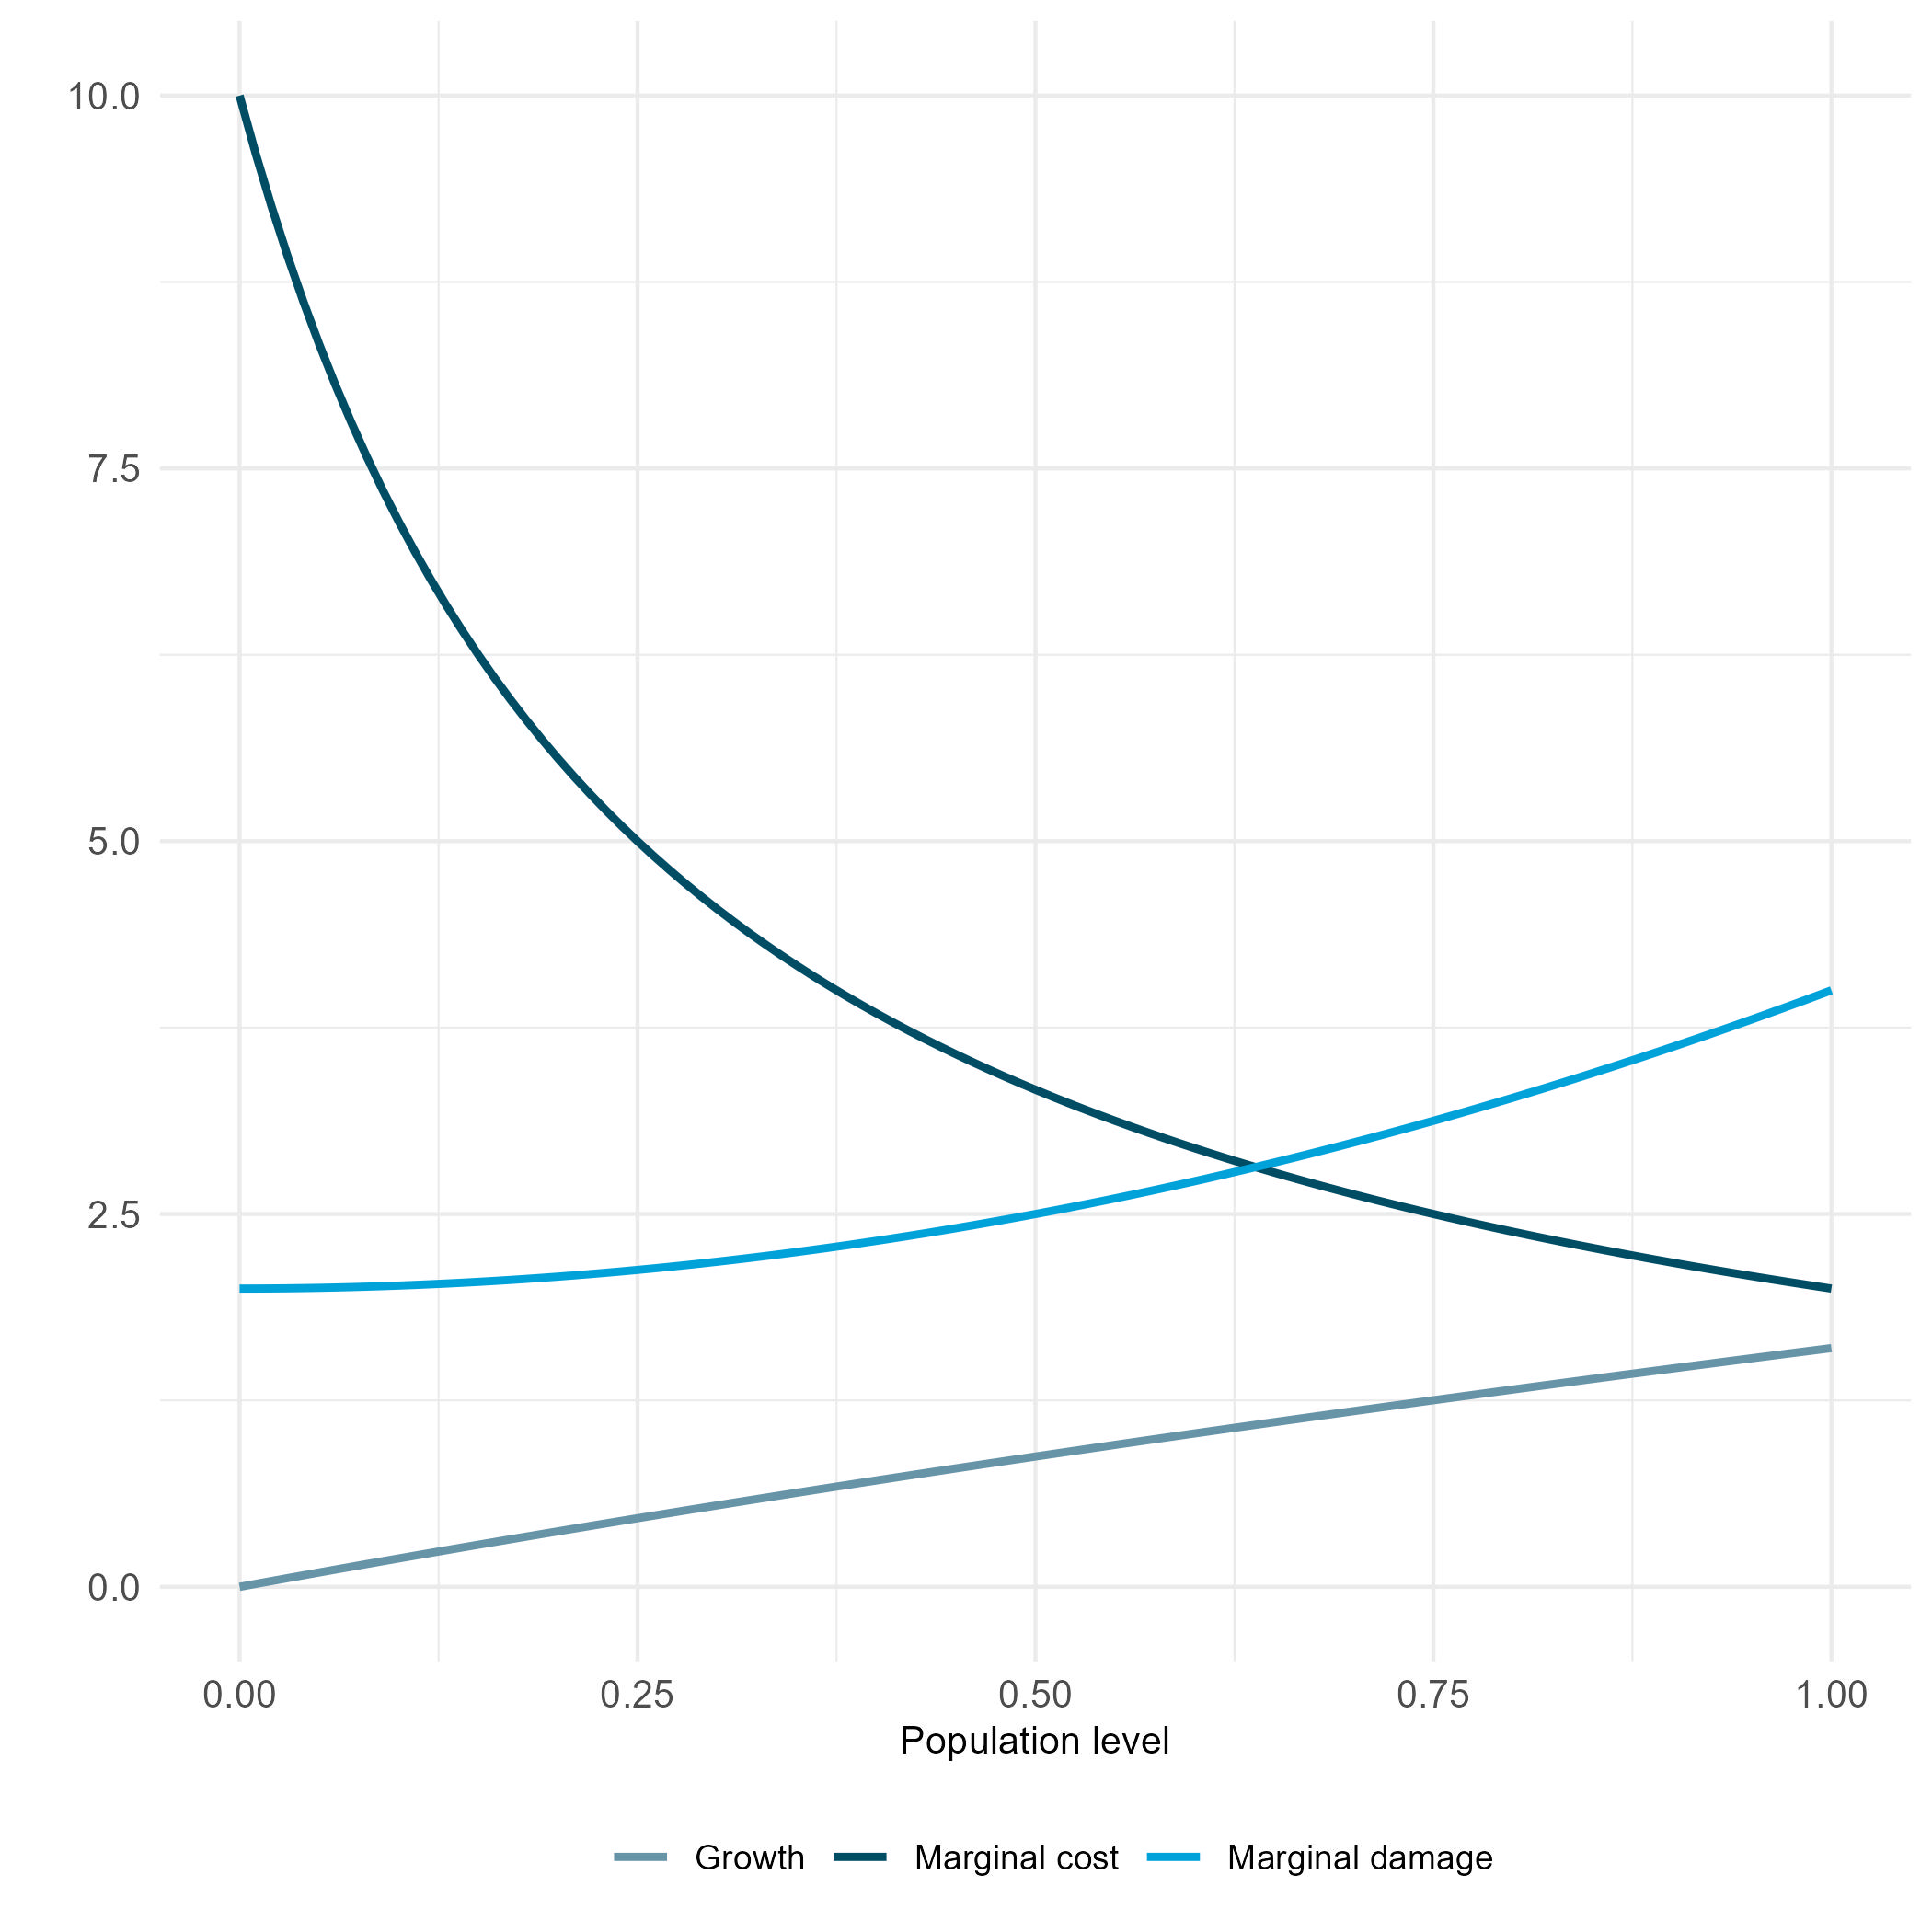
\includegraphics[width = .8\textwidth]{figures/fences/baseline_functions.jpg}
	\caption{Illustration of baseline functions for numerical illustration}
\end{figure}


%\subsection{Proof of concavity}
%Starting from the first order conditions in equations \ref{eq:foc_control_non_cooperative} and \ref{eq:foc_fence_non_cooperative} and omitting time subscripts in $t$ (but remaining in $t+1$), the second order derivatives are :

%\begin{align}
%\frac{\partial^2 C_i}{\partial e_i^2} &= -c_i'(e_i) + k'_i(e_i) +\delta\left[g_i''(e_i)(1-d_{ij}(f_i, f_j))c_i(X_{it+1}) + \left(g'_i(e_i)(1- d_{ij}(f_i, f_j))\right)^2 c'_i(X_{it+1})\right]\\
%
%\frac{\partial^2 C_i}{\partial f_i^2} &= \gamma_i'(f_i) + \delta \left[g_i(e_i)\left(-\frac{\partial d_{ij}}{\partial f_i}c_i'(X_{it+1}) - \frac{\partial^2 d_{ij}}{\partial f_i^2}c_i(X_{it+1}) \right) + g_j(e_j)\left(\frac{\partial d_{ji}}{\partial f_i}c_i'(X_{it+1} + \frac{\partial ^2 d_{ji}}{\partial f_i^2}c_i(X_{it+1})\right) \right]\\
%
%\frac{\partial^2 C_i}{\partial e_i \partial f_i} &= \delta g_i'(e_i)\left[-\frac{\partial d_{ij}}{\partial f_i}\left(c_i(X_{it+1}) + c_i'(X_{it+1})g_i(e_i)\right) + c_i(X_{it+1}) \frac{\partial d_{ji}}{\partial f_i}g_j(e_j)\right]\\
%
%\frac{\partial ^2 C_i}{\partial f_i \partial e_i} &= -\frac{\partial d_{ij}}{\partial f_i}\delta g_i'(e_i)\left[c_i(X_{it+1}) + g_i(e_i)c_i'(X_{it+1})(1 - d_{ij}(f_i, f_j) \right]
%\end{align}



\subsection{Effect of dispersal on optimal residual stock}

\cite{costello_private_2017} define a set of first order conditions such that : 
\begin{equation}
c_i(e_i) - k_i(e_i) = \delta g'_i(e_i)((1-d_{ij}c_i(X_{it+1}) + d_{ji}c_j(X_{jt+1})
\end{equation}
These conditions define an optimal solution as long as the second order condition is met, stemming from the convexity of the returns on control i.e. as long as : 
\begin{align*}
SOC_i = k_i'(e_{it}) - c_i(e_{it}) &+ \delta g_i''(e_{it})(d_{ij}c_i(X_{it+1}) + (1-d_{ij})c_i(X_{it+1})) \\ 
&+\delta (g_i(e_{it}))^2 (d_{ij}^2 c_j(X_{jt+1}) + (1- d_{ij})^2 c_i(X_{it+1})>0
\end{align*}

From the first order conditions, we can determine the effect of changing dispersal patterns on optimal residual stock : 

\begin{align}
&\frac{d}{d d_{ij}}\left(k_i(e_{it}) - c_i(e_{it})+ \delta g_i'(e_{it})[d_{ij} c_j(X_{jt+1})  (1-d_{ij})c_i(X_{it+1})]\right) = 0 \nonumber \\
\iff 
& (k_i'(e_{it}) - c_i(e_{it})) \frac{\partial e_{it}}{\partial d_{ij}}  \\
& + \delta g''_i(e_{it})(d_{ij}c_j(X_{jt+1}) + (1-d_{ij})c_i(X_{it+1})\frac{\partial e_{it}}{\partial d_{ij}} \\
& + \delta g_i'(e_{it})(c_j(X_{jt+1}) - c_i(X_{it+1}))  \label{eq:foc_dispersal_direct_effect} \\
& + \delta g_i'(e_{it})[(1-d_{ij})c_i'(X_{it+1}) \frac{d X_{it+1}}{d d_{ij}} + d_{ij}c_j'(X_{jt+1})\frac{d X_{jt+1}}{d d_{ij}}) = 0
\label{eq:foc_dispersal_raw}
\end{align}
The variation in residual stock is such that the current changes in marginal cost and damages caused by the change in optimal residual stock, the change in the future cost caused by (i) the growth of the population migrating along current dispersal patterns, (ii) the marginal population flow change without adjustments from the optimal stock and (iii) the marginal cost of changes in future population levels are equal. The change in future populations are :
\begin{align*}
\frac{dX_{it+1}}{d d_{ij}} &= \frac{d}{d d_{ij}} \left( (1-d_{ij})g_i(e_{it}) + d_{ji} g_j(e_{jt}) \right)\\
& = \left( - g_i(e_{it}) + (1-d_{ij})\frac{\partial e_{it}}{\partial d_{ij}} g_i'(e_{it}) + d_{ji}\frac{\partial e_{jt}}{\partial d_{ij}}g_j'(e_{jt}) \right)\\
\\
\frac{dX_{jt+1}}{d d_{ij}} & \frac{d}{d d_{ij}} \left( (1-d_{ji})g_j(e_{jt}) + d_{ij} g_i(e_{it}) \right)\\
 &= \left( g_i(e_{it}) + d_{ij}\frac{\partial e_{it}}{\partial d_{ji}} g_i'(e_{it}) + (1-d_{ji})\frac{\partial e_{jt}}{\partial d_{ji}}g_j'(e_{jt}) \right)
\end{align*}
The changes in future population feature a direct effect from the change in dispersal, and an indirect effect from the marginal growth effect that follows the adaptation of optimal residual stock to changes in dispersal patterns. Reformulating equation \ref{eq:foc_dispersal_raw} : 

\begin{equation}
\frac{\partial e_{it}}{\partial d_{ij}} = \frac{1}{\Omega_i}\left(\frac{\partial e_{jt}}{\partial d_{ij}}\gamma_i + \eta_i\right)
\end{equation}
Where : 
\begin{align*}
\Omega_i &= k_i'(e_{it}) - c_i'(e_{it}) 
+ \delta g_i''(e_{it}) \left( d_{ij}c_i(X_{it+1}) + (1-d_{ij})c_i(X_{it+1}) \right) \\ 
&\quad + \delta (g_i'(e_{it}))^2 \left( d_{ij}^2 c_j(X_{jt+1}) + (1- d_{ij})^2 c_i(X_{it+1}) \right) = SOC_i >0 \\
\gamma_i &= - \delta g_i'(e_{it}) g_j'(e_{jt}) \left( (1-d_{ij}) d_{ji} c_j'(X_{jt+1}) + d_{ji}(1-d_{ij})c_i'(X_{it+1}) \right)>0\\
\eta_i &= - \delta g_i'(e_{it})(c_j(X_{jt+1}) - c_i(X_{it+1}) +  g_i(e_{it}) \left( d_{ij}c_j'(X_{jt+1}) - (1-d_{ij})c_i'(X_{it+1}) \right)
\end{align*}
The sign of $\eta_i$ depends on cost differential incurred by a change in the dispersal rate alone, and the marginal cost difference caused by the adaptation of the population. It is the joint effect of changing the dispersal and keeping the population unchanged, and changing the population while leaving the dispersal unchanged. 
Using the same method : 
\begin{equation}
\frac{\partial e_{it}}{\partial d_{ji}} = \frac{1}{\Omega_i}\left(\frac{\partial e_{jt}}{\partial d_{ji}}\gamma_i + \Phi_i\right)
\end{equation}
Where : 
\begin{align*}
\Phi_i = - \delta g_i'(e_{it}) g_j(e_{jt}) \left( (1-d_{ij})c_i'(X_{it+1}) - d_{ij}c_j'(X_{jt+1}) \right)
\end{align*}
$\Phi_i$ and $\eta_i$ differ because of the absence of a direct effect as in equation \ref{eq:foc_dispersal_direct_effect}. 
\\
These partial derivatives form a system such that : 
\begin{equation}
\begin{cases}
\frac{\partial e_{it}}{\partial d_{ij}} &= \frac{1}{\Omega_i}\left(\frac{\partial e_{jt}}{\partial d_{ij}}\gamma_i + \eta_i\right)\\
\frac{\partial e_{jt}}{\partial d_{ij}} &= \frac{1}{\Omega_j}(\frac{\partial e_{it}}{\partial d_{ij}}\gamma_j + \Phi_j)\\
\frac{\partial e_{it}}{\partial d_{ji}} &= \frac{1}{\Omega_i}(\frac{\partial e_{jt}}{\partial d_{ji}}\gamma_i + \Phi_i)\\
\frac{\partial e_{jt}}{\partial d_{ji}} &= \frac{1}{\Omega_j}\left(\frac{\partial e_{it}}{\partial d_{ji}}\gamma_j + \eta_j\right)
\end{cases}
\end{equation}

Therefore : 

\begin{align}
\frac{\partial e_{it}}{\partial d_{ij}} = \frac{\Phi_j \gamma_i + \eta_i \Omega_j}{\Omega_i \Omega_j - \gamma_i\gamma_j} \\
\frac{\partial e_{it}}{\partial d_{ji}} = \frac{\gamma_i \eta_j + \Omega_j \Phi_i}{\Omega_i \Omega_j - \gamma_i \gamma_j}
\end{align}

The sign of these two expressions is ambiguous, as all elements can be both positive and negative. We restrict our attention to the analysis of $\Phi$ and $\eta$ to uncover insights into the behavior of $e_{it}$ and $e_{jt}$. When residual stock is large, or the discount factor is low, it is safe to assume that the denominator is positve (ultimately, the sign of the denominator depends on the relative magnitude of $c_i'(X_{it+1}), c_j'(X_{jt+1})$ and $c_i(X_{it+1}), c_j(X_{jt+1})$). The sign of the partial derivatives therefore depends on the numerator.\\

\subsubsection{Effect of outbound dispersal in patch $j$}

Focus on $\frac{\partial e_{it}}{\partial d_{ij}}$ and the case where it is unambiguously negative, such that $\Phi_j<0 \text{ and } \eta_i<0$:
\begin{align*}
&
\begin{cases}
&((1-d_{ji})c_j'(X_{jt+1}) -d_{ji}c_i'(X_{it+1})>0\\
& (c_j(X_{jt+1}) - c_i(X_{it+1}) + g_i(e_{it}) (d_{ij}c_j'(X_{jt+1}) - (1-d_{ij})c_i'(X_{it+1}))>0
\end{cases}
\\
&
\begin{cases}
\left|\frac{1 - d_{ji}}{d_{ji}}c_j'(X_{jt+1})\right| > \left|c_i'(X_{it+1})\right| \\
g_i(e_{it}) \left( [ c_j(X_{jt+1}) + d_{ij}c_j'(X_{jt+1}) ] - \left[ c_i(X_{it+1}) + (1 - d_{ij})c_i'(X_{it+1}) \right] \right) > 0
\end{cases}
\end{align*}

First, for homogeneous linear marginal costs, these are always 0: the movement of optimal dispersal depends on the sensitivity of the marginal cost. Moreover, the first term holds for small values of $d_{ji}$ and homogeneous costs, but does not hold for larger values as $\lim_{d_{ji} \to 1} \frac{(1-d_{ji}}{d_{ji}}=0$. The second tirm holds for specific realms of the elasiticities of marginal costs (i.e. $\epsilon_i = \frac{c_i'(X_{it+1}}{c_i(X_{it+1}}$). Rewriting the second condition :
\begin{equation}
\left(  c_j(X_{jt+1})[1-d_{ij}|\epsilon_j|] - c_i(X_{it+1})[1-(1-d_{ij})|\epsilon_i|]\right)>0
\end{equation}
Hence, for low values of $d_{ij}$, this tends to hold, while it no longer does for dispersals. 

This heuristic demonstration tends to show that for moderate values of $d_{ij}$,$\frac{\partial e_{it}}{\partial d_{ij}}<0$ and for larger values, $\frac{\partial e_{it}}{\partial d_{ij}}>0$. 

\subsubsection{Effect of inbound dispersal change in patch $i$}

This second part is ongoing work. 


\subsubsection{Numerical illustration of the effect of dispersal on optimal residual stock}
\begin{figure}[H]
    \centering
    \begin{subfigure}{0.8\textwidth}
        \centering
        \includegraphics[width=\textwidth]{figures/fences/derivative_escapements_dAB_interior_baseline.jpg}
        \caption{Interior solutions}
        \label{fig:escapement_derivative_interior}
    \end{subfigure}
    \hfill
    \begin{subfigure}{0.8\textwidth}
        \centering
        \includegraphics[width=\textwidth]{figures/fences/derivative_escapements_dAB_baseline.jpg}
        \caption{All solutions}
        \label{fig:escapement_derivative_overall}
    \end{subfigure}
    \caption{Evolution of optimal residual stock with respect to dispersal from $A$ to $B$ ($d_{AB}$)}
    \label{fig:overall}
\end{figure}

\subsection{Proof of changes in value following change in dispersal}
In the case of interior solutions, the optimal residual stock is defined by equation \ref{eq:foc_costello} as $e^*_{it}$. In this case, the Bellman equation can be rewritten as : 
\begin{equation*}
V(\mathbf{X}_t, \mathbf{D}) = \sum_{i\in\{A,B\}}\left(\int_{0}^{e^*_{it}} k_i(s)ds + \int_{e_{it}^*}^{X_{it}} c_i(s)ds \right) + \delta V(\mathbf{X}^*, \mathbf{D})
\end{equation*}

Assuming we remain in the realm of interior solutions, we can use the enveloppe theorem:

\begin{align*}
\frac{\partial V}{\partial d_{ij}} = \sum_{i\in \{A,B\}} \frac{\partial }{\partial e_{it}}\left(\int_{0}^{e^*_{it}} k_i(s)ds + \int_{e_{it}^*}^{X_{it}} c_i(s)ds\right) \frac{\partial e_{it}^*}{\partial d_{ij}} + \sum_{i\in \{A,B\}}\frac{\partial V}{\partial X_{it+1}}\frac{\partial X_{it+1}}{\partial d_{ij}}
\end{align*}
The first derivatives with respect to $e_{it}$ are, by definition, equal to 0, as $e_{it}^*$ is determined by the first-order conditions. Given that
\[
\frac{\partial V}{\partial X_{it+1}} = c_i(X_{it+1})
\]
and
\[
\frac{\partial X_{ijt+1}}{\partial d_{ij}} = \left( - g_i(e_{it}) + (1 - d_{ij}) g_i'(e_{it}) \frac{\partial e_{it}}{\partial d_{ij}} + d_{ji} \frac{\partial e_{jt}}{\partial d_{ij}} \right),
\]
we obtain equation \ref{eq:variation_of_value_function}.

\subsection{Proof of socially optimal management with fences and control}

Let the Bellman equation be : 

\begin{equation}
V(\mathbf{X}_t) = \min_{\{e_{it}, f_{it}\}_{i \in \{A,B\}}}\left( \sum_{i\in\{A,B\}}\int_{0}^{e_{it}} k_i(s)ds + \int_{e_{it}}^{X_{it}} c_i(s)ds \right) + \delta V(\mathbf{X}_{t+1})
\end{equation}

\subsubsection{Interior conditions for socially optimal management}
\label{appendix:proof_stock_independence_foc}
Taking the first order conditions with respect to residual stock and fencing in each patch $i$ : 

\begin{align*}
&- c_i(e_{it}) + k_i(e_{it}) + \delta \sum_{j}\frac{\partial V}{\partial e_{it}}(X_{jt+1} \leq 0 \\
\iff & - c_i(e_{it}) + k_i(e_{it}) + \delta \left(  \sum_j c_j(X_{jt+1}\frac{\partial X_{jt+1}}{\partial e_{it}}\right) \leq 0\\
\iff & - c_i(e_{it}) + k_i(e_{it}) + \delta \left( \sum_j c_j(X_{jt+1} d_{jit+1}(f_{jt}, f_{it}) g_i'(e_{it})\right) \leq 0 \\
\end{align*}
Using the fact that $\frac{\partial V}{\partial X_{it+1}} = c_i(X_{it+1})$ and $\frac{\partial X_{jt+1}}{\partial e_{it}} = d_{ijt+1}(f_{jt}, f_{it})g_i'(e_{it})$, and the fact that $d_{iit+1}=(1-d_{ijt+1}(f_{jt},f_{it})$ setting the FOC at 0 yields equation \ref{eq:optimal_harvest}. As $e_{it}$ is interior, it does not depend on $X_{it}$. 

For interior fencing levels : 
\begin{align*}
&\kappa_i + \delta \sum_j \frac{\partial V}{\partial X_{jt+1}}\frac{\partial X_{jt+1}}{\partial f_{it}}\leq 0\\
\iff & \kappa_i + \delta \sum_j \left( c_j(X_{jt+1}) \frac{\partial X_{jt+1}}{\partial f_{it}}\right) \leq 0
\end{align*}
Using the fact that $\frac{\partial X_{jt+1}}{\partial f_{it}} = \left( \frac{\partial d_{jit+1}}{\partial f_{it}}g_i(e_{it})\right)$ and $d_{iit+1} = (1 - d_{ijt+1}(f_{jt},f_{it})$ yields equation \ref{eq:optimal_fencing}. As $f_{it}$ depends on $e_{it}$, which is independent of $X_{it}$, $f_{it}$ is independent of $X_{it}$. 
\\
These first order conditions are sufficient, if the second order conditions hold i.e $det(H)>0$ where $H$ is the Hessian matrix of the problem. I focus on this case, but further analysis is needed to ensure this holds. It is likely to hold in the case of convex control costs, but several equilibria may arise in the presence of homogeneous costs, damages and growth.

\subsubsection{Absence of fencing in the absence of spatial heterogeneity}
\label{appendix:proof_absence_fencing}
Using homogeneous linear marginal costs of control : 

\begin{align*}
k_i(e_{it})& = c - \delta g'_i(e_{it})\left[c + d_{ijt+1}(f_{it}, f_{it})(c - c)) \right]\\
\Rightarrow & c - k_i(e_{it}) = \delta g'_i(e_{it}) c
\end{align*}

And optimal fencing in patch $i$ towards patch $j$ is : 
\begin{align*}
\kappa_i & = \delta\left(\frac{\partial d_{ij+1}}{\partial f_{it}} g_i(e_{it}) - \frac{\partial d_{jit+1}}{\partial f_{it}}g_j(e_{jt})\right) \big(c - c\big)\\
\Rightarrow \kappa_i & = \delta\left(\frac{\partial d_{ij+1}}{\partial f_{it}} g_i(e_{it}) - \frac{\partial d_{jit+1}}{\partial f_{it}}g_j(e_{jt})\right)\times 0 = 0
\end{align*}
Hence, $f_{it}= 0$ for $i \in \{A, B\}$

If costs are heterogeneous (in the proof, I use linear costs, but this holds for any costs) but there is no dispersal : 
\begin{align*}
k_i(e_{it})& = c_i - \delta g'_i(e_{it})\left[c_i + d_{ijt+1}(f_{it}, f_{it})(c_j - c_i)) \right]\\
\Rightarrow & c_i - k_i(e_{it}) = \delta g'_i(e_{it}) c_i
\end{align*}

And optimal fencing in patch $i$ towards patch $j$ is : 
\begin{align*}
&\kappa_i = \delta\left(\frac{\partial d_{ij+1}}{\partial f_{it}} g_i(e_{it}) - \frac{\partial d_{jit+1}}{\partial f_{it}}g_j(e_{jt})\right) \big(c - c\big)\\
\Rightarrow \kappa_i& = \delta\left(0 \times g_i(e_{it}) - 0 \times g_j(e_{jt})\right)\times 0 = 0
\end{align*}

\subsubsection{Optimal management with heterogeneous costs and exclusionary fencing}
Proposition \ref{prop:exclusion_optimal} holds as a direct application of $\frac{\partial d_{ijt+1}}{\partial f_{it}}=0$.

\subsubsection{Optimal management with heterogeneous costs, trap and exclusionary effects}
\label{appendix:heterogenous_cost_trap_exclusion}
Rewrite equation \ref{eq:optimal_fencing}, and notice that the first-order condition only holds if for some values $\tilde{e}_{it}, \tilde{e}_{jt}, \tilde{f}_{it}$, and $\tilde{f}_{jt}$, equation \ref{eq:optimal_fencing_both_effects_ci} holds. Further, notice that if dispersal functions are identical, $\frac{\partial d_{ABt+1}}{\partial f_{Bt}} = \frac{\partial d_{BAt+1}}{\partial f_{At}}$ and $\frac{\partial d_{ABt+1}}{\partial f_{At}} = \frac{\partial d_{BAt+1}}{\partial f_{Bt}}$. Finally, if $c_A>c_B$, the first-order conditions yield: 
\begin{align*}
&\kappa_A = \delta \left( \frac{\partial d_{ABt+1}}{\partial f_{At}} g_A(e_{At}) - \frac{\partial d_{BAt+1}}{\partial f_{Bt}} g_B(e_{Bt}) (c_A - c_B) \right) \\
&\kappa_B > \frac{\partial d_{ABt+1}}{\partial f_{Bt}} = \frac{\partial d_{BAt+1}}{\partial f_{At}} \underbrace{(c_B - c_A)}_{<0}
\end{align*}

Therefore, fencing can only happen in one patch. 
\subsection{Non cooperative equilibrium}
\subsubsection{Interior MPNE}
\label{appendix:interior_mpne}
Using the Bellman equation, the first order condition for $\bar{e}_{it}$ yield : 

\begin{align*}
&- c_i + k_i(e_{it}) + \delta \frac{\partial V_i}{\partial e_{it}}\leq 0 \\
\iff &  - c_i + k_i(e_{it}) + \delta c_i g_i'(e_{it}) (1 - d_{ijt+1}(f_{it},f_{jt})\leq 0\\
\Rightarrow &  c_i + k_i(\bar{e}_{it}) + \delta c_i g_i'(\bar{e}_{it}) (1 - d_{ijt+1}(\bar{f}_{it},\bar{f}_{jt}) = 0
\end{align*}
Using the fact that $\frac{\partial V_i}{\partial X_{it+1}} = c_i$ and $\frac{\partial V_i}{\partial X_{jt+1}}=0$ and $\frac{\partial X_{it+1}}{\partial e_{it}} = (1 - d_{ijt+1}(f_{it},f_{jt}))g_i'(e_{it})$. Turning to $\bar{f}_{it}$, recognizing that $\frac{\partial X_{it+1}}{\partial f_{it}} = g_j(e_{jt})\frac{\partial d_{jit+1}}{\partial f_{it}} - \frac{\partial d_{ijt+1}}{\partial f_{it}}g_i(e_{it})$:
\begin{align*}
& \kappa_i + \delta \frac{\partial V_i}{\partial X_{it+1}}\frac{\partial X_{it+1}}{\partial f_{it}}\leq 0\\
\Rightarrow & \kappa + \delta c_i \left( g_j(\bar{e}_{jt})\frac{\partial d_{jit+1}}{\partial f_{it}} - \frac{\partial d_{ijt+1}}{\partial f_{it}}g_i(\bar{e}_{it})\right) = 0
\end{align*}
These conditions are sufficient assuming that the second order conditions are satisfied, i.e. $det(H)>0$ where $H$ is the Hessian matrix of the problem.

\clearpage
%% Conceptual challenges



{\footnotesize
\bibliographystyle{abbrvnat}
\bibliography{bibliography_these}
}
\cleardoublepage